\documentclass[man,floatsintext]{apa6}
\usepackage{lmodern}
\usepackage{amssymb,amsmath}
\usepackage{ifxetex,ifluatex}
\usepackage{fixltx2e} % provides \textsubscript
\ifnum 0\ifxetex 1\fi\ifluatex 1\fi=0 % if pdftex
  \usepackage[T1]{fontenc}
  \usepackage[utf8]{inputenc}
\else % if luatex or xelatex
  \ifxetex
    \usepackage{mathspec}
  \else
    \usepackage{fontspec}
  \fi
  \defaultfontfeatures{Ligatures=TeX,Scale=MatchLowercase}
\fi
% use upquote if available, for straight quotes in verbatim environments
\IfFileExists{upquote.sty}{\usepackage{upquote}}{}
% use microtype if available
\IfFileExists{microtype.sty}{%
\usepackage{microtype}
\UseMicrotypeSet[protrusion]{basicmath} % disable protrusion for tt fonts
}{}
\usepackage{hyperref}
\hypersetup{unicode=true,
            pdftitle={Registered Replication Report on Fischer, Castel, Dodd, and Pratt (2003)},
            pdfauthor={Lincoln J Colling, Dénes Szűcs, Damiano De Marco, Krzysztof Cipora, Rolf Ulrich, Hans-Christoph Nuerk, Mojtaba Soltanlou, Donna Bryce, Sau-Chin Chen, Philipp Alexander Schroeder, Dion T Henare, Christine K Chrystall, Paul M Corballis, Daniel Ansari, Celia Goffin, H Moriah Sokolowski, Peter JB Hancock, Ailsa E Millen, Stephen RH Langton, Kevin J Holmes, Mark S Saviano, Tia A Tummino, Oliver Lindemann, Rolf A Zwaan, Jiří Lukavský, Adéla Becková, Marek A Vranka, Simone Cutini, Irene Cristina Mammarella, Claudio Mulatti, Raoul Bell, Axel Buchner, Laura Mieth, Jan Philipp Röer, Elise Klein, Stefan Huber, Korbinian Moeller, Brenda Ocampo, Juan Lupiáñez, Javier Ortiz-Tudela, Juanma De la fuente, Julio Santiago, Marc Ouellet, Edward M Hubbard, Elizabeth Y Toomarian, Remo Job, Barbara Treccani, \& Blakeley B McShane},
            pdfborder={0 0 0},
            breaklinks=true}
\urlstyle{same}  % don't use monospace font for urls
\usepackage[style=apa]{biblatex}

\addbibresource{cited.bib}
\usepackage{graphicx,grffile}
\makeatletter
\def\maxwidth{\ifdim\Gin@nat@width>\linewidth\linewidth\else\Gin@nat@width\fi}
\def\maxheight{\ifdim\Gin@nat@height>\textheight\textheight\else\Gin@nat@height\fi}
\makeatother
% Scale images if necessary, so that they will not overflow the page
% margins by default, and it is still possible to overwrite the defaults
% using explicit options in \includegraphics[width, height, ...]{}
\setkeys{Gin}{width=\maxwidth,height=\maxheight,keepaspectratio}
\IfFileExists{parskip.sty}{%
\usepackage{parskip}
}{% else
\setlength{\parindent}{0pt}
\setlength{\parskip}{6pt plus 2pt minus 1pt}
}
\setlength{\emergencystretch}{3em}  % prevent overfull lines
\providecommand{\tightlist}{%
  \setlength{\itemsep}{0pt}\setlength{\parskip}{0pt}}
\setcounter{secnumdepth}{0}
% Redefines (sub)paragraphs to behave more like sections
\ifx\paragraph\undefined\else
\let\oldparagraph\paragraph
\renewcommand{\paragraph}[1]{\oldparagraph{#1}\mbox{}}
\fi
\ifx\subparagraph\undefined\else
\let\oldsubparagraph\subparagraph
\renewcommand{\subparagraph}[1]{\oldsubparagraph{#1}\mbox{}}
\fi

%%% Use protect on footnotes to avoid problems with footnotes in titles
\let\rmarkdownfootnote\footnote%
\def\footnote{\protect\rmarkdownfootnote}


  \title{Registered Replication Report on Fischer, Castel, Dodd, and Pratt (2003)}
    \author{\textbf{Lincoln J Colling}\textsuperscript{1}, \textbf{Dénes
Szűcs}\textsuperscript{1}, Damiano De Marco\textsuperscript{1, 12},
Krzysztof Cipora\textsuperscript{2}, Rolf Ulrich\textsuperscript{2},
Hans-Christoph Nuerk\textsuperscript{2}, Mojtaba
Soltanlou\textsuperscript{2}, Donna Bryce\textsuperscript{2}, Sau-Chin
Chen\textsuperscript{3}, Philipp Alexander Schroeder\textsuperscript{4},
Dion T Henare\textsuperscript{5}, Christine K
Chrystall\textsuperscript{5}, Paul M Corballis\textsuperscript{5},
Daniel Ansari\textsuperscript{6}, Celia Goffin\textsuperscript{6}, H
Moriah Sokolowski\textsuperscript{6}, Peter JB
Hancock\textsuperscript{7}, Ailsa E Millen\textsuperscript{7}, Stephen
RH Langton\textsuperscript{7}, Kevin J Holmes\textsuperscript{8}, Mark S
Saviano\textsuperscript{8}, Tia A Tummino\textsuperscript{8}, Oliver
Lindemann\textsuperscript{9}, Rolf A Zwaan\textsuperscript{9}, Jiří
Lukavský\textsuperscript{10}, Adéla Becková\textsuperscript{11}, Marek A
Vranka\textsuperscript{11}, Simone Cutini\textsuperscript{12}, Irene
Cristina Mammarella\textsuperscript{12}, Claudio
Mulatti\textsuperscript{12}, Raoul Bell\textsuperscript{13}, Axel
Buchner\textsuperscript{13}, Laura Mieth\textsuperscript{13}, Jan
Philipp Röer\textsuperscript{14, 2}, Elise Klein\textsuperscript{15},
Stefan Huber\textsuperscript{15}, Korbinian
Moeller\textsuperscript{15,2}, Brenda Ocampo\textsuperscript{16}, Juan
Lupiáñez\textsuperscript{17}, Javier Ortiz-Tudela\textsuperscript{17},
Juanma De la fuente\textsuperscript{17}, Julio
Santiago\textsuperscript{17}, Marc Ouellet\textsuperscript{17}, Edward M
Hubbard\textsuperscript{18}, Elizabeth Y Toomarian\textsuperscript{18},
Remo Job\textsuperscript{19}, Barbara Treccani\textsuperscript{19}, \&
Blakeley B McShane\textsuperscript{20}}
    \date{}
  
  
\shorttitle{Registered Replication Report on Fischer, Castel, Dodd, and Pratt (2003)}
\affiliation{
\vspace{0.5cm}
\textsuperscript{1} Department of Psychology, University of Cambridge\\\textsuperscript{2} Department of Psychology, University of Tübingen\\\textsuperscript{3} Department of Human Development and Psychology, Tzu-Chi University\\\textsuperscript{4} Department of Psychiatry and Psychotherapy, University of Tübingen\\\textsuperscript{5} School of Psychology, University of Auckland\\\textsuperscript{6} Department of Psychology \& Brain and Mind Institute, The University of Western Ontario\\\textsuperscript{7} Psychology, Faculty of Natural Sciences, University of Stirling, Stirling, UK\\\textsuperscript{8} Department of Psychology, Colorado College\\\textsuperscript{9} Department of Psychology, Education \& Child Studies, Erasmus University Rotterdam, Netherlands\\\textsuperscript{10} Institute of Psychology of the Czech Academy of Sciences\\\textsuperscript{11} Department of Psychology, Faculty of Arts, Charles University\\\textsuperscript{12} Department of Developmental Psychology, University of Padova\\\textsuperscript{13} Department of Experimental Psychology, Heinrich Heine University Düsseldorf\\\textsuperscript{14} Department of Psychology and Psychotherapy, Witten/Herdecke University\\\textsuperscript{15} Leibniz-Institut für Wissensmedien, Tübingen\\\textsuperscript{16} School of Psychology, The University of Queensland\\\textsuperscript{17} Research Center for Mind, Brain, and Behavior, University of Granada\\\textsuperscript{18} Department of Educational Psychology, University of Wisconsin-Madison\\\textsuperscript{19} Department of Psychology and Cognitive Science, University of Trento\\\textsuperscript{20} Kellogg School of Management, Northwestern University}
\usepackage{csquotes}
\usepackage{upgreek}
\captionsetup{font=singlespacing,justification=justified}

\usepackage{longtable}
\usepackage{lscape}
\usepackage{multirow}
\usepackage{tabularx}
\usepackage[flushleft]{threeparttable}
\usepackage{threeparttablex}

\newenvironment{lltable}{\begin{landscape}\begin{center}\begin{ThreePartTable}}{\end{ThreePartTable}\end{center}\end{landscape}}

\makeatletter
\newcommand\LastLTentrywidth{1em}
\newlength\longtablewidth
\setlength{\longtablewidth}{1in}
\newcommand{\getlongtablewidth}{\begingroup \ifcsname LT@\roman{LT@tables}\endcsname \global\longtablewidth=0pt \renewcommand{\LT@entry}[2]{\global\advance\longtablewidth by ##2\relax\gdef\LastLTentrywidth{##2}}\@nameuse{LT@\roman{LT@tables}} \fi \endgroup}


\renewcommand\appendixname{Supplementary Results}
\usepackage{subcaption}
\usepackage{caption}
\usepackage{makecell}
\DeclareLanguageMapping{english}{english-apa}
\DeclareBibliographyCategory{asterisk}
\renewbibmacro*{begentry}{\ifcategory{asterisk}{\ensuremath{\ast}}{}}
\newcommand*{\nocitemeta}[1]{\nocite{#1}\addtocategory{asterisk}{#1}}
\usepackage{fontspec}
\setmainfont{Tinos}
\usepackage{float}
\floatplacement{figure}{htp}

\authornote{

Correspondence concerning this article should be addressed to
\textbf{Lincoln J Colling} E-mail:
\href{mailto:lincoln@colling.net.nz}{\nolinkurl{lincoln@colling.net.nz}}}

\abstract{
The attentional spatial-numerical association of response codes
(Att-SNARC) effect (Fischer, Castel, Dodd, \& Pratt, 2003)---the finding
that participants are quicker to detect left-side targets when the
targets are preceded by small numbers and quicker to detect right-side
targets when they are preceded by large numbers---has been used as
evidence for \emph{embodied} number representations and to support
strong claims about the link between number and space (e.g., a mental
number line). We attempted to replicate Experiment 2 of Fischer et al.
by collecting data from 1105 participants at 17 labs. Across all 1105
participants and four interstimulus-interval conditions, the proportion
of times the effect we observed was positive (i.e., directionally
consistent with the original effect) was .50. Further, the effects we
observed both within and across labs were minuscule and incompatible
with those observed by Fischer et al. Given this, we conclude that we
failed to replicate the effect reported by Fischer et al. In addition,
our analysis of several participant-level moderators (finger-counting
habits, reading and writing direction, handedness, and mathematics
fluency and mathematics anxiety) revealed no substantial moderating
effects. Our results indicate that the Att-SNARC effect cannot be used
as evidence to support strong claims about the link between number and
space.


}

  
\note{The final version of this paper is 
Advances in Methods and Practices in Psychological Science \url{https://doi.org/10.1177/2515245920903079}}


\usepackage{amsthm}
\newtheorem{theorem}{Theorem}[section]
\newtheorem{lemma}{Lemma}[section]
\theoremstyle{definition}
\newtheorem{definition}{Definition}[section]
\newtheorem{corollary}{Corollary}[section]
\newtheorem{proposition}{Proposition}[section]
\theoremstyle{definition}
\newtheorem{example}{Example}[section]
\theoremstyle{definition}
\newtheorem{exercise}{Exercise}[section]
\theoremstyle{remark}
\newtheorem*{remark}{Remark}
\newtheorem*{solution}{Solution}
\begin{document}

\begin{center}
AUTHOR ACCEPTED VERSION
\end{center}

\begin{center}
The final version is available at 
{\bf Advances in Methods and Practices in Psychological Science} \url{https://doi.org/10.1177/2515245920903079}
\end{center}

\maketitle

\section{Introduction}\label{introduction}

A foundational issue in cognitive science is the question of how people
represent concepts. Classical approaches to cognitive science,
exemplified by Fodor's \autocite*{Fodor1975} \emph{language-of-thought
hypothesis} and Newell and Simon's \autocite*{Newell1976}
\emph{physical-symbol-systems hypothesis}, view representations as
abstract or amodal and as distinct from sensorimotor processing. In
contrast to these traditional views, a range of other views that go
under labels such as \emph{embodied}, \emph{situated}, or
\emph{grounded} cognition maintain that representations (a) are
intimately linked to sensorimotor processing \autocite[see, e.g.,][ for
an overview]{Wilson2002six}, (b) are analog rather than symbolic, and
(c) represent by resembling their targets in some sense \autocites[e.g.,
see][]{Gladzijewski2017}{Williams2018}.

One area of research that has provided a wealth of empirical findings
valuable for debates about this issue has been numerical cognition. In
fact, \textcite{Fischer2011em} referred to numerical cognition as the
\enquote{prime example of embodied cognition.} In particular, they
pointed to tasks examining spatial-numerical associations to make their
case.

Researchers have long reasoned that numbers might be represented in a
spatially organized manner (Galton, 1880), for example, as a
\emph{mental number line} \autocite[e.g.,][]{Restle:1970km}. Key support
for this notion comes from a series of nine parity-judgment experiments
conducted by \textcite{Dehaene:1993fc}. In their experiments,
\textcite{Dehaene:1993fc} asked participants to judge whether a number
was odd or even and reported that responses to large numbers were faster
when participants pressed a right-hand key rather than a left-hand key,
whereas the opposite was true for small numbers. They labeled this
number-magnitude-by-response-side interaction the spatial-numerical
association of response codes (SNARC) effect.

In these experiments, there was no standard with which to compare the
presented number. Consequently, whether a particular number was
responded to more quickly with the left hand or the right hand was not
determined by the absolute magnitude of the number, but rather by the
relative magnitude of the number within a stimulus set. Thus, the number
5 was responded to more quickly with the left hand when it appeared in a
set of numbers ranging from 4 to 9 but more quickly with the right hand
when it appeared in a set of numbers ranging from 0 to 5
\autocites[e.g.,][]{Dehaene:1993fc}{Fias:1996ms}.

\textcite{Dehaene:1993fc} reported that the effect was dependent on
neither the handedness of participants nor the hand used to make the
response, but instead depended on the side of space of the response:
When participants' hands were crossed, responses to small numbers were
quicker with the right hand than with the left \autocite[however,
see,][]{Woods:2006cp}. Nonetheless, \textcite{Dehaene:1993fc} did report
that the effect was dependent on participants' reading and writing
direction. Specifically, although they reported finding the effect in
experiments with French participants, who had experience reading and
writing from left to right, they also reported failing to find the
effect in an experiment with Iranian participants, who had experience
reading and writing from right to left (see \textcite{Shaki:2009ch} and
\textcite{Zebine}). Together, the results from the nine experiments
reported in \textcite{Dehaene:1993fc} were taken to support the idea of
a mental number line and the association of numbers of increasing
magnitude with the left-to-right axis of external space.

Although the SNARC effect appears to be robust (see
\textcite{Wood:2008rev} and \textcite{Toomarian:2018rev} for recent
reviews), the great range of findings has resulted in debate about
mechanism. One such debate concerns whether the SNARC effect is produced
by early, response-independent mechanisms or whether processes at the
stage of response selection are responsible. According to theories that
place the origin of the SNARC effect at an early stage, the mere
observation of a number should be sufficient to activate the spatial
code because the spatial code is intimately connected to the numerical
representation. Consequently, these theories make the strongest claims
about the link between number and space. Theories that place the origin
of the SNARC effect at the response-selection stage, however, make
weaker claims about the connection between number and space. As
\textcite{PecherBoot:2011} noted, if the response-selection stage gives
rise to the SNARC effect, then no underlying spatial-numerical
representation need be assumed.

Most recent work has tended to support the notion that the
response-selection stage is the locus of the SNARC effect. In
particular, Keus and colleagues have used both behavioral
\autocite{Keus:2005ho} and psychophysiological \autocite{Keus:2005jh}
evidence to argue in favor of a later, response-related origin of the
SNARC effect. Further support comes from a computational model that
relies on task-dependent conceptual coding of the number at a stage
distinct from the numerical representation itself
\autocite{Gevers:2006model}.

In addition, response-polarity-related accounts break the link between a
number, space, and the SNARC effect. For example,
\textcite{Proctor:2006jv} argued that on binary classification tasks,
items in the task set are coded as being positive or negative in
polarity. Response selection can then be facilitated when there is a
structural overlap between the polarity of the item (the number in the
case of the SNARC effect) and the response. Thus, perceptual or
conceptual overlap between the stimulus and response dimensions is not
required for the SNARC effect to occur. In short,
\textcite{Gevers:2006model} model and \textcite{Proctor:2006jv} account
do not rely on the notion of a mental number line or sensorimotor-linked
representations.

A range of empirical findings support these types of accounts. For
example, \textcite{Santens:2008} reported that SNARC-like effects can be
produced when left-right responses are replaced with unimanual close-far
responses; small numbers are associated with close responses, and large
numbers are associated with far responses. Further,
\textcite{Landy:2008} reported that verbal \enquote{yes} and
\enquote{no} responses on a parity-judgment task were facilitated by
large numbers and small numbers, respectively.

Finally, still other researchers have argued in favor of a working
memory account of the SNARC effect. For example, in an experiment
reported by \textcite{vanDijck:2011kk}, participants performed a
fruit/vegetable classification task after having been encouraged to
store the stimuli as an ordered set in working memory. Specifically, a
sequence of fruit and vegetable names was displayed in the center of the
computer screen, and participants were tested on the order of the items.
Then, in a subsequent classification task, responses to items that had
appeared early in the sequence were faster if made with the left hand
rather than the right hand, and responses to items that had appeared
later in the sequence were faster if made with the right hand rather
than the left hand. The authors argued that this working memory account
can also explain why SNARC-like effects emerge for other kinds of
ordinal sequences, such as months of the year \autocite{Gevers:2003je}
or days of the week \autocite{Gevers:2004gj}, as well as why
spatial-numerical associations can be moderated by giving participants
instructions to associate numbers with positions on a clockface (1--5 on
the right and 6--10 on the left) rather than on a ruler \autocite[1--5
on the left and 6--10 on the right;][]{Bachtold:1998}.

Given that several competing accounts of the SNARC effect exist and that
many of these accounts do not require a mental number line, one may
doubt whether spatial-numerical associations provide evidence for
anything like \enquote{embodied} number representations or number
representations that are intimately linked with space. However, there is
evidence that does support an early, response-independent locus for the
SNARC effect and thus does provide support for the notion of a mental
number line and spatially linked number representation---the modified
version of Posner's \autocite*{Posner} attentional cuing task developed
by \textcite{Fischer:2003ju}. In Fischer et al.'s experiment,
participants were asked to press a single response button whenever a
lateralized target, a white circle, appeared, regardless of whether it
appeared on the left or the right. The target was always preceded by
either a small number (1 or 2) or a large number (8 or 9), which was
unrelated to the subsequent location of the target. Because the response
was not lateralized, response-related effects were not possible. Results
from this paradigm were consistent with the SNARC effect, as
participants were quicker to detect left-side targets when they were
preceded by small numbers and quicker to detect right-side targets when
they were preceded by large numbers, at least when the numbers and
targets were separated by an interstimulus interval (ISI) between 250
and 1000 ms. This finding---named the attentional SNARC (Att-SNARC)
effect---suggests that viewing a number can cue spatial attention either
to the left or to the right depending on the magnitude of the number.

Because the Att-SNARC effect is strong evidence in favor of an early,
response-independent locus for the mechanism underlying the SNARC
effect, the Att-SNARC effect plays a crucially important role in
adjudicating debates about the origin of the SNARC effect and the nature
of number representations. As a result, Fischer et al.'s original
finding has been extremely influential (e.g., cited 746 times according
to Google Scholar as of May 15, 2020). However, subsequent attempts to
replicate the effect have produced a wide array of results.

\textcite{Galfano:2006cu} reported a so-called statistically significant
effect for left-side targets when the data were aggregated over ISI
conditions of 500 and 800 ms and a one-tailed test was employed,
estimate = 6 ms, \emph{t}(25) = 1.75, \emph{p} = .046 (reported as
\emph{p} = .04). They also reported a statistically significant effect
for right-side targets when the data were aggregated over these two ISI
conditions and a one-tailed test was employed, but the claimed
statistical significance reflected a reporting error, estimate = 5 ms,
\emph{t}(25) = 1.59, \emph{p} = .062 (reported as \emph{p} = .04).
Although it is possible to obtain a point estimate for each of the ISI
conditions with the data aggregated over the left- and right-side
targets (500-ms ISI: 8 ms; 800-ms ISI: 4 ms), the corresponding
variances and test statistics for these estimates were not reported and
cannot be obtained from what was reported.

\textcite{Ristic:2006cr} reported a statistically significant effect
when the data were aggregated over six ISI conditions ranging from 350
to 800 ms and over the left- and right-side targets, estimate = 3.79 ms
(unreported; obtained via digitization of the figure), \emph{F}(1, 17) =
5.48, \emph{p} = .032 (reported as \emph{p} \textless{} .05). Although
it is possible, via digitization of the figure, to obtain a point
estimate for each of the six ISI conditions with the data aggregated
over the left- and right-side targets (350-ms ISI: 11.24 ms; 400-ms ISI:
2.81 ms; 500-ms ISI: --1.44 ms; 600-ms ISI: 6.17 ms; 700-ms ISI: 6.05
ms; 800-ms ISI: --2.17 ms), the corresponding variances and test
statistics for these estimates were not reported and cannot be obtained
from what was reported.

\textcite{Dodd:2008dv} reported a statistically significant effect when
the data were aggregated over three ISI conditions ranging from 250 to
750 ms and over the left- and right-side targets, but the claimed
statistical significance reflected a reporting error, estimate = 5.5 ms
(unreported), \emph{F}(1, 29) = 4.05. \emph{p} = .054 (reported as
\emph{p} \textless{} .05). They also reported statistically significant
effects for the 500-ms ISI condition for left-side targets, estimate =
16 ms, \emph{t}(29) = 2.48, \emph{p} = .010 (reported as \emph{p}
\textless{} .05), and for right-side targets, estimate = 6 ms,
\emph{t}(29) = 2.34, \emph{p} = .013 (reported as \emph{p} \textless{}
.05). Although it is possible to obtain a point estimate for each of the
three ISI conditions with the data aggregated over the left- and
right-side targets (250-ms ISI: 6 ms; 500-ms ISI: 11 ms; 750-ms ISI:
--0.5 ms), the variances and test statistics for these estimates were
not reported and cannot be obtained from what was reported.

\textcite{Salillas2008} reported a so-called statistically
nonsignificant effect for a 450-ms ISI condition when the data were
aggregated over the left- and right-side targets, estimate = 7.5 ms,
\emph{F}(1, 11) = 1.3, \emph{p} = .28 (reported as \enquote{ns}).
Additionally, \textcite{Ranzini2009} reported a statistically
nonsignificant effect when the data were aggregated over three ISI
conditions ranging from 300 to 500 ms and over the left- and right-side
targets, estimate = 3 ms (unreported; obtained via digitization of the
figure), \emph{F}(1, 14) = 4.1, \emph{p} = .06. Point estimates and
variances and test statistics for such estimates for the three ISI
conditions with the data aggregated over the left- and right-side
targets were not reported and cannot be obtained from what was reported.

More recently, \textcite{vanDijck2014} reported a statistically
nonsignificant effect when the data were aggregated over four ISI
conditions ranging from 250 to 1000 ms and over the left- and right-side
targets, estimate = 1 ms (unreported; obtained via digitization of the
figure), reported \emph{F(1, 42)} \textless{} 1.05, reported \emph{p}
\textgreater{} .37. Point estimates and variances and test statistics
for such estimates for the four ISI conditions with the data aggregated
over the left- and right-side targets were not reported and cannot be
obtained from what was reported. In a second experiment,
\textcite{vanDijck2014} also reported a statistically nonsignificant
effect when the data were aggregated over three ISI conditions ranging
from 100 to 700 ms and over the left- and right-side targets, estimate =
--2.5 ms (unreported; obtained via digitization of the figure),
\emph{F}(1, 28) = 2.94, \emph{p} = .097 (no estimates were reported).
Point estimates and variances and test statistics for such estimates for
the three ISI conditions with the data aggregated over the left- and
right-side targets were not reported and cannot be obtained from what
was reported.

\textcite{Zanolie:2014jr} reported a statistically nonsignificant effect
when the data were aggregated over four ISI conditions ranging from 250
to 1000 ms and over the left- and right-side targets, estimate = 0.5 ms
(unreported; obtained via digitization of the figure), \emph{F}(1, 19) =
0.03, \emph{p} = .863. Although it is possible to obtain a point
estimate for each of the four ISI conditions with the data aggregated
over the left- and right-side targets (250-ms ISI: --1 ms; 500-ms ISI: 2
ms; 750-ms ISI: 5 ms; 1000-ms ISI: --4 ms), the variances and test
statistics for these estimates were not reported and cannot be obtained
from what was reported. In a second experiment,
\textcite{Zanolie:2014jr} also reported a statistically nonsignificant
effect when the data were aggregated over the same four ISI conditions
and over the left- and right-side targets, estimate = --1.5 ms
(unreported; obtained via digitization of the figure), \emph{F}(1, 23) =
0.17, \emph{p} = .686. Although it is possible to obtain a point
estimate for each of the four ISI conditions with the data aggregated
over the left- and right-side targets (250-ms ISI: --2 ms; 500-ms ISI: 5
ms; 750-ms ISI: --3 ms; 1000-ms ISI: --6 ms), the variances and test
statistics for these estimates were not reported and cannot be obtained
from what was reported.

Finally, \textcite{Fattorini2015} reported a statistically
nonsignificant effect when the data were aggregated over 500-ms and
700-ms ISI conditions and over the left- and right-side targets,
estimate = 2 ms (unreported; obtained via digitization of the figure),
\emph{F}(1, 59) = 1.69, \emph{p} = .20. Point estimates and variances
and test statistics for such estimates for the two ISI conditions with
the data aggregated over the left- and right-side targets were not
reported and cannot be obtained from what was reported. In a second
experiment, \textcite{Fattorini2015} also reported a statistically
nonsignificant effect when the data were aggregated over four ISI
conditions ranging from 250 to 1000 ms and over the left- and right-side
targets, estimate = --1.75 ms (unreported; obtained via digitization of
the figure), \emph{F}(1, 31) = 1.5, \emph{p} = .22. Although it is
possible to obtain a point estimate for each of the four ISI conditions
with the data aggregated over the left- and right-side targets (250-ms
ISI: --2 ms; 500-ms ISI: --1 ms; 750-ms ISI: --2 ms; 1000-ms ISI: --2
ms), the variances and test statistics for these estimates were not
reported and cannot be obtained from what was reported.

A natural approach to assessing these various attempts to replicate the
Att-SNARC effect would involve synthesizing the evidence across all
published studies of the effect via meta-analysis. This would allow for,
among other things, the estimation of an overall average effect size,
the heterogeneity in effect sizes across studies, and the effects of
potential moderators at the study level or otherwise. However, this
approach is complicated because (a) the statistical significance (or
nonsignificance) of a study's results typically affects whether or not
the study is published, which results in a set of published studies that
is not representative, and (b) meta-analytic results are biased when the
set of studies analyzed is not representative
\autocites{McSBocHan16}{ioannidis:eff}. Instead, the Registered
Replication Report (RRR) format pursued in the present study provides an
ideal means of assessing the Att-SNARC effect because in an RRR, results
from all participating labs are included in the meta-analysis regardless
of their statistical significance or nonsignificance. Further,
preregistration of the primary hypotheses and statistical analyses
mitigates some potential biases.

An additional benefit of the RRR format is that it allows for the
investigation of potential moderators not previously considered, which
might shed new light on mechanism and perhaps also the wide array of
results observed in the various attempts to replicate the Att-SNARC
effect. Consequently, in addition to replicating the experimental
protocol of Fischer et al., we investigated several variables that could
potentially moderate the Att-SNARC effect: finger-counting habits,
reading and writing direction, handedness, and mathematics ability and
mathematics anxiety (see Fischer
\autocites{Fischer:2006er}{Fischer:2008bv}, \textcite{Fischer:2014kz},
\textcite{Georges:2016gn}, and \textcite{Shaki:2009ch} for details and
conjectures).

Before proceeding, we note that alternative accounts of the effect
reported by Fischer et al. have been suggested. These include, for
example, accounts based on working memory \autocite{vanDijck2014}. We
also note that manipulations that make explicit associations between
number and space have been able to produce Att-SNARC-like effects
\autocite[e.g.,][experiment 3]{Fattorini2015}. Because these alternative
accounts and additional manipulations have theoretical implications for
the Att-SNARC effect that differ that originally proposed and our focus
is on the latter, we do not consider them here.

\section{Disclosures}\label{disclosures}

\subsection{Preregistration}\label{preregistration}

This study was preregistered. All relevant documentation is available on
the Open Science Framework (OSF) at \url{https://osf.io/he5za/}

\subsection{Data, materials, and online
resources}\label{data-materials-and-online-resources}

The data and materials are available on OSF at
\url{https://osf.io/he5za/}. Links to the lab-specific pages of all
participating labs are available on OSF at \url{https://osf.io/7zyxj}.
Data and scripts to re-create the manuscript are available on a
companion website at \url{http://git.colling.net.nz/attentional_snarc/}.
An archived version of the companion website is available at
\url{https://doi.org/10.5281/zenodo.3738555}.

\subsection{Reporting}\label{reporting}

We report how we determined our sample size, all data exclusions, all
manipulations, and all measures in the study.

\subsection{Ethical approval}\label{ethical-approval}

All participating labs obtained ethical approval in accordance with
their local requirements, and the research was carried out in according
with the Declaration of Helsinki.

\section{Methods}\label{methods}

\subsection{Sample size}\label{sample-size}

Each participating lab was required to provide a target sample size no
smaller than 60 participants and a stopping rule (see the lab-specific
pages for details). We chose 60 participants as the minimum because, as
required for RRRs, it provides high power conditional on a hypothetical
assumed effect size of 0.92 for a one-tailed test at α = .05,
conditional on an effect size of 0.4 on the standardized Cohen's
\emph{d} scale, about the midpoint of previously published estimates.
This value corresponds to a raw effect size of 6 ms assuming a
between-participants standard deviation of 15 ms, again about the
midpoint of previously published estimates.

Because of time constraints, not all labs were able to reach the minimum
target of 60 participants (see Table 1 for the sample size achieved by
each lab). However, given the sample sizes actually achieved, and again
conditional on an effect size of 0.4 on the standardized Cohen's
\emph{d} scale, a statistically significant effect would be expected in
93\% of the labs (i.e., about 16). Thus, if 0.4 is a reasonable estimate
of the effect size and there are no substantial moderators of the
effect, statistically significant effects would be expected not only at
the meta-analytic level but also at the level of the individual lab.

\subsection{Materials}\label{materials}

The participating labs all had (a) a testing station, such as a room or
a cubicle, where participants could undertake the experiment without
distraction; (b) a computer for presenting stimuli and recording
responses; (c) a chin rest or similar device to ensure that participants
remained a set distance from the computer monitor; and (d) a tape
measure used to calibrate distance from the screen. Five labs also
optionally made use of an eye tracker to record participants' eye
movements during the attentional-cuing task (see the lab-specific pages
for details).

An instruction booklet detailing how to perform the setup and
calibration procedure and the finger-counting assessment was provided to
the labs. These materials were initially written in English, but each
lab conducted the experiment in the predominant language of its locale.
Thus, the experiment was also conducted in German, Dutch, Czech,
Spanish, Italian, and Chinese. All materials were translated from
English into these other languages and then independently
back-translated into English to ensure accuracy.

All materials including translations are available on OSF (see
\url{https://osf.io/7zyxj/}). To perform analyses, we used R
\autocite[Version 3.5.1;][]{R-base} and the R packages \emph{bindrcpp}
\autocite[Version 0.2.2;][]{R-bindrcpp}, \emph{checkmate}
\autocite[Version 1.8.5;][]{R-checkmate}, \emph{dplyr} \autocite[Version
0.7.6;][]{R-dplyr}, \emph{forcats} \autocite[Version
0.3.0;][]{R-forcats}, \emph{forestplot} \autocite[Version
1.7.2;][]{R-forestplot}, \emph{ggplot2} \autocite[Version
3.0.0;][]{R-ggplot2}, \emph{glue} \autocite[Version 1.3.0;][]{R-glue},
\emph{kableExtra} \autocite[Version 0.9.0;][]{R-kableExtra},
\emph{knitr} \autocite[Version 1.20;][]{R-knitr}, \emph{lme4}
\autocite[Version 1.1.18.1;][]{R-lme4}, \emph{magick} \autocite[Version
1.9;][]{R-magick}, \emph{magrittr} \autocite[Version
1.5;][]{R-magrittr}, \emph{Matrix} \autocite[Version
1.2.14;][]{R-Matrix}, \emph{nlme} \autocite[Version 3.1.137;][]{R-nlme},
\emph{papaja} \autocite[Version 0.1.0.9842;][]{R-papaja}, \emph{purrr}
\autocite[Version 0.2.5;][]{R-purrr}, \emph{pwr} \autocite[Version
1.2.2;][]{R-pwr}, \emph{R.matlab} \autocite[Version
3.6.2;][]{R-R.matlab}, \emph{readr} \autocite[Version
1.1.1;][]{R-readr}, \emph{reticulate} \autocite[Version
1.10;][]{R-reticulate}, \emph{stringr} \autocite[Version
1.3.1;][]{R-stringr}, \emph{tibble} \autocite[Version
1.4.2;][]{R-tibble}, \emph{tidyr} \autocite[Version 0.8.1;][]{R-tidyr},
and \emph{tidyverse} \autocite[Version 1.2.1;][]{R-tidyverse}.

\subsection{Procedure}\label{procedure}

We employed an experimental paradigm based on Experiment 2 of
\textcite{Fischer:2003ju}. We chose Experiment 2 over Experiment 1
because Experiment 2 had fewer ISI conditions and because the results
were statistically significant in a greater proportion of the
conditions. Before starting data collection, each lab performed a
monitor calibration procedure using a supplied calibration script. This
procedure involved measuring the viewing distance from the computer
monitor and the size of standard stimuli presented on the screen (see
\url{https://osf.io/2m4ad/} for details). After participants provided
informed consent, they were seated in front of the monitor with their
chin placed in a chin rest that was located a fixed distance from the
monitor (set during the calibration procedure), and then data collection
commenced.

The standard trial structure, which was identical to that of Fischer et
al. and did not include timing modifications for the eye tracker (see
the Eye-Tracking Protocol subsection for details), is shown in Figure
\ref{fig:Trial}. The initial display on each trial consisted of a
centrally located white fixation point (0.2° diameter) flanked by two
white outline boxes (1° \(\times\) 1°), all on a black background. The
centers of the boxes were located 5° from the center of the fixation
point. This initial display was shown for 500 ms. Next, a digit (1, 2,
8, or 9; height of 0.75°) replaced the fixation point for a fixed
duration of 300 ms. After the digit was removed, the fixation point
reappeared. Finally, a circular white target (0.7° diameter) appeared in
either the left- or the right-side box after a variable duration (250
ms, 500 ms, 750 ms, or 1000 ms) on target trials, and no target appeared
on catch trials.

Target trials ended after a response was made or 1000 ms after the onset
of the target, whichever came first. Catch trials ended 1000 ms after
the digit was removed. Trials advanced automatically, separated by an
intertrial interval of 1000 ms.

Participants responded to the appearance of the target by pressing the
space bar with their preferred hand. When a participant responded before
the target appeared or responded on a catch trial, the trial ended, and
the following warning appeared: \enquote{Too quick! Please wait until
the target appears in a box before pressing SPACE} {[}English
version{]}. When a participant failed to respond on a target trial, the
following warning was presented: \enquote{Too slow! Please press SPACE
as soon as the target appears.} Participants who erred on more than 5\%
of trials were excluded from analyses.

Participants performed a total of 800 trials (640 target trials and 160
catch trials), split into five blocks of 160 trials each, with 128
target trials and 32 catch trials per block; the trials in each block
were evenly divided across the four ISI conditions, four digits, and two
target locations, and the order of presentation was random.













\begin{figure}
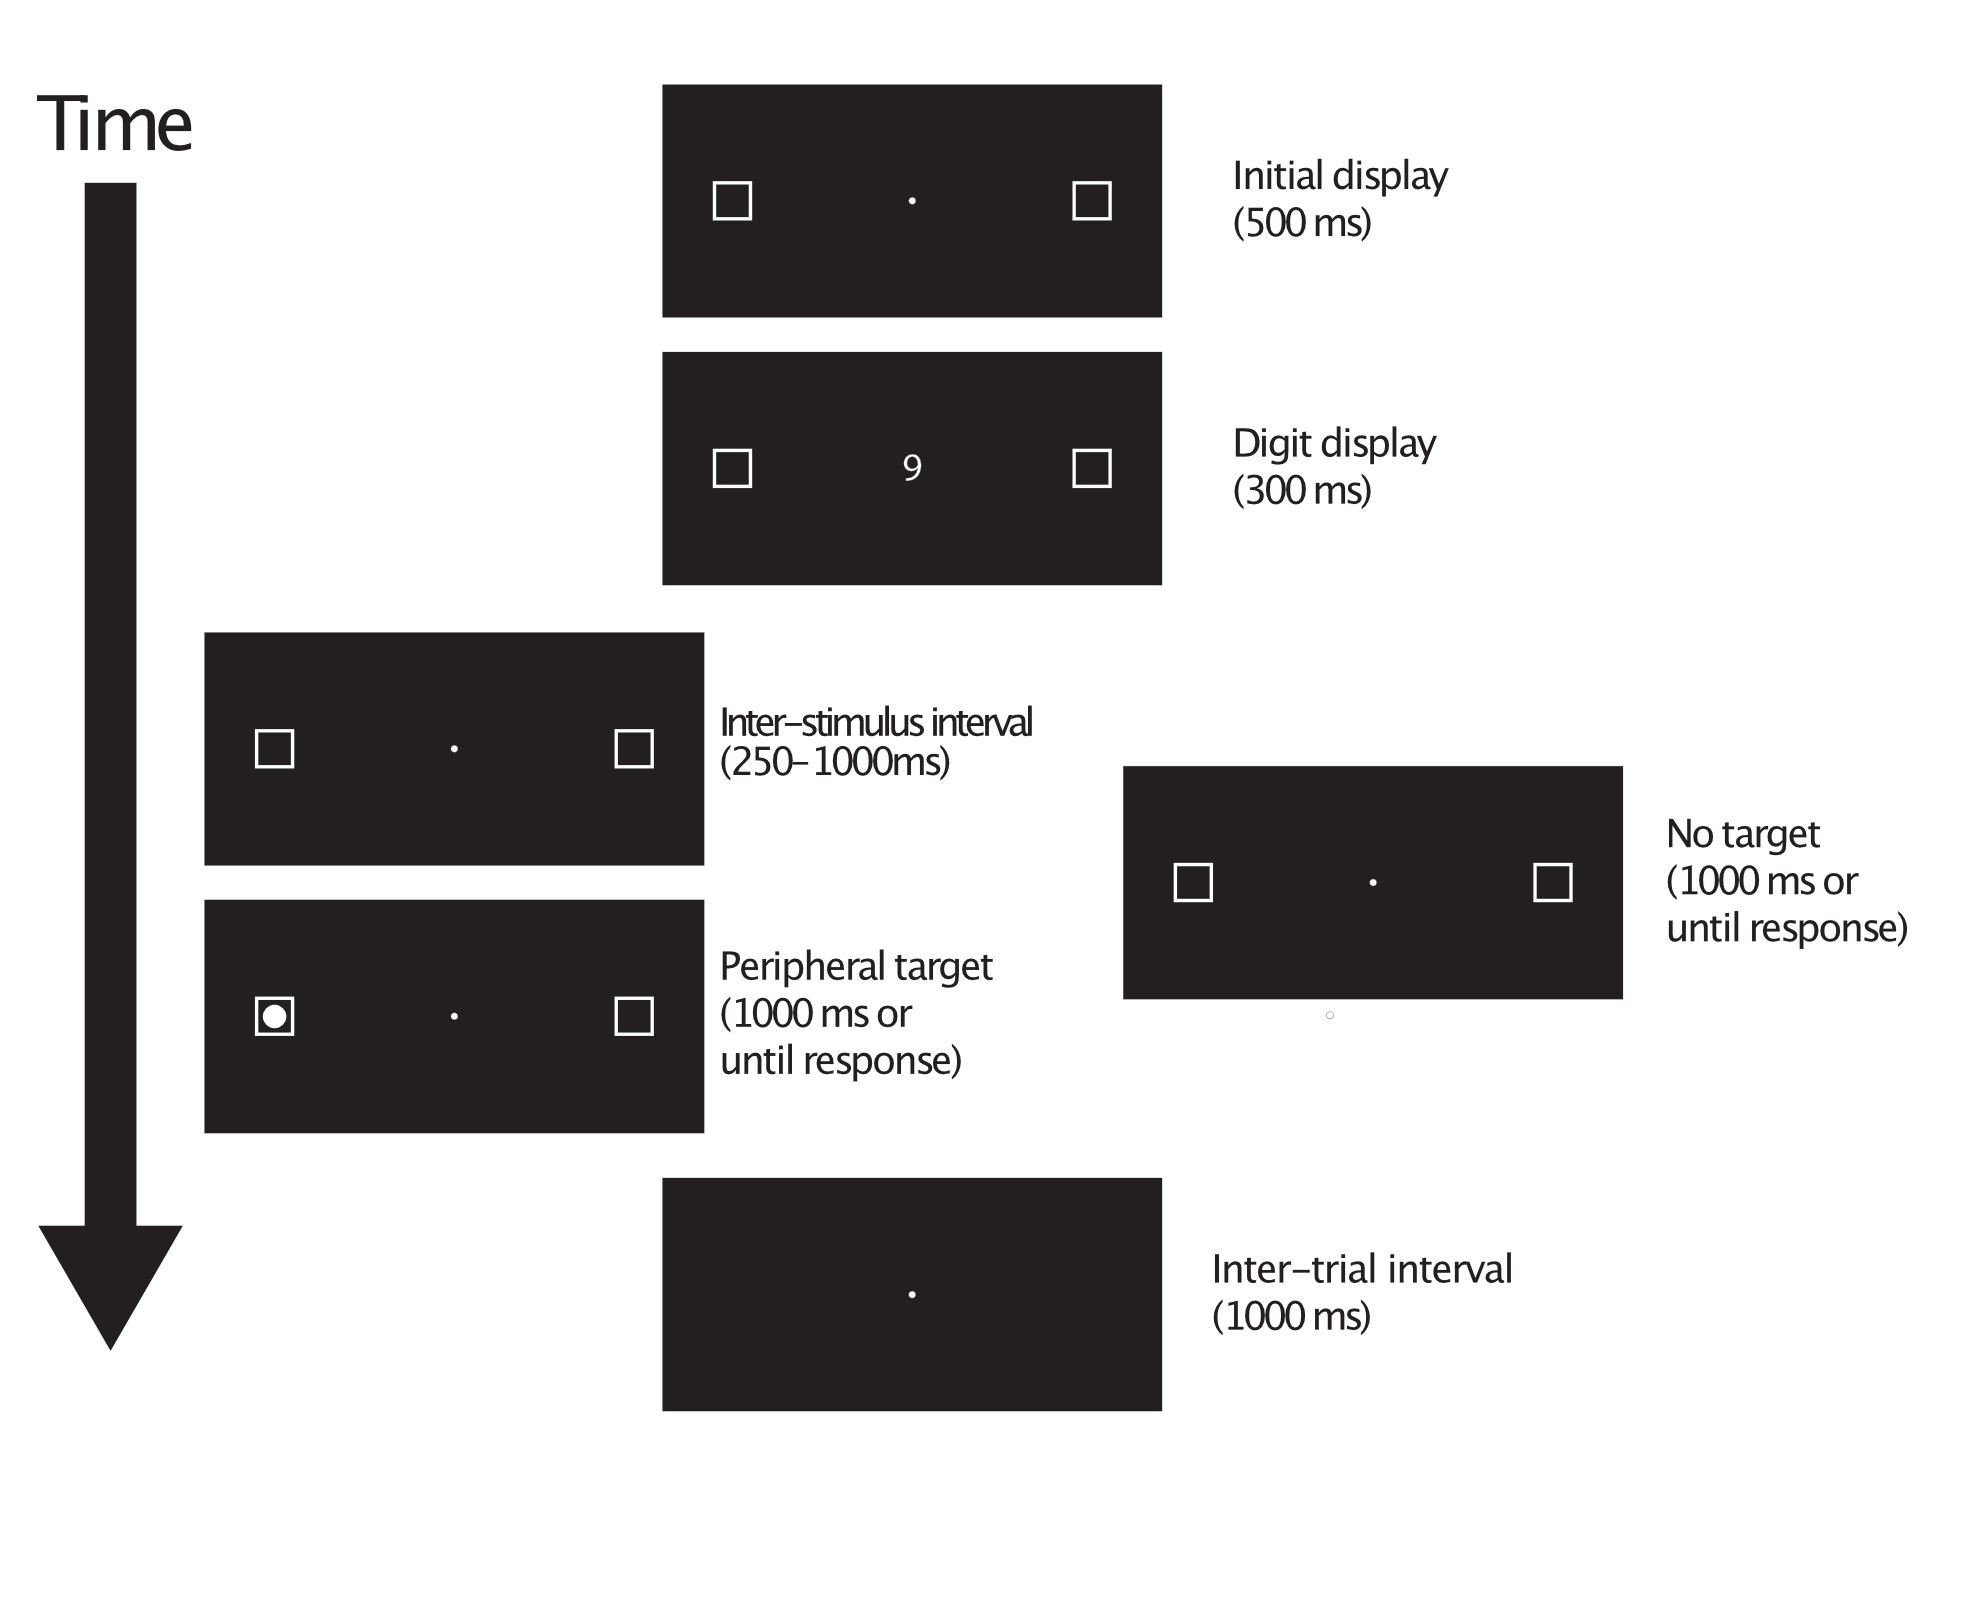
\includegraphics[width=\textwidth]{trialstructure} \caption{Trial structure for target trials and catch trials. The
initial display on each trial consisted of a centrally located white
fixation point flanked by two white outline boxes, all on a black
background. Next, a digit replaced the fixation point. After the digit
was removed, the fixation point reappeared. Finally, a circular white
target appeared in either the left- or the right-side box after a
variable duration on target trials, and no target appeared on catch
trials. Target trials ended after a response was made or 1000 ms after
the onset of the target, whichever came first. Catch trials ended 1000
ms after the digit was removed. Trials advanced automatically, separated
by an intertrial interval of 1000 ms.}\label{fig:Trial}
\end{figure}

\subsection{Eye-tracking protocol}\label{eye-tracking-protocol}

Code implementing an eye-tracking protocol using an EyeLink 1000 (SR
Research, Ottawa, Ontario, Canada) eye tracker was provided to all labs
and is available at Github
(\url{https://github.com/ljcolling/FischerRRR-eyetracking}). Of the five
labs that optionally made use of an eye tracker, one used a different
eye tracker; this lab has provided information regarding deviations from
the standard protocol on its lab-specific page. The standard nine-point
grid was used for calibration and validation at the start of each block
and when required during a block. The start of a trial was triggered
after the detection of 500 ms of stable fixation within a 2° box
centered on the fixation point. If the system could not detect a stable
fixation within a 2000-ms time window, the calibration process was
repeated. After the digit was presented, and before the target appeared,
the gaze position was monitored, and any deviations outside a 1° box
centered on the fixation point were recorded. Any deviations toward the
lateral boxes that exceeded 2° resulted in the trial being marked as
contaminated. These trials were excluded from primary analyses; however,
they were analyzed separately in an attempt to determine any possible
effect of eye movements on the results.

\subsection{Finger counting}\label{finger-counting}

To assess finger-counting fluency, we used a task derived from that
developed by \textcite{Lucidi:2014gn}. Participants were asked to read
aloud four sentences while counting the number of syllables in each.
Because reading aloud prevents verbalizing counting, most participants
needed to resort to finger counting while sounding out the syllables.
For each sentence, the experimenter recorded the first finger and first
hand the participant used. Although most participants used their fingers
for the task, some participants adopted a different strategy.
Participants who failed to engage in finger counting after two sentences
were prompted to do so. Details of the prompting were recorded in lab
logs (see the lab-specific pages for details).

The results from the finger-counting task were used to place
participants into five groups: consistent left-starters, consistent
right-starters, inconsistent left-starters, inconsistent right-starters,
and others. This classification was determined not only by participants'
hand choices, but also by how consistently they engaged in finger
counting. The consistent left-starters and consistent right-starters
included those participants who counted using a hand on all four
occasions and started on the same hand on at least three of them. The
inconsistent left-starters and inconsistent right-starters included
participants who counted using a hand on two or three occasions and
started on the same hand on at least two of them. The \emph{other} group
included all remaining participants (e.g., those who did not count on
their fingers, those who counted on their fingers only once, and those
who counted an equal number of times with each hand).

\subsection{Reading/writing direction}\label{readingwriting-direction}

To assess reading and writing direction, we used a simple question
asking participants if they had experience with languages that are
written exclusively from left to right (e.g., English and German), with
languages that are not written exclusively from left to right (e.g.,
Hebrew), or with languages of both types (see
\url{https://osf.io/dqnkq/} for details). For the Chinese version of
this question, participants were asked if they had experience with
languages that are usually written horizontally, with languages that are
usually written vertically, or with languages of both types (see
\url{https://osf.io/r3fhx/} for details). Responses to this question
were used to place participants into two groups: exclusively
left-to-right readers-writers and not exclusively left-to-right
readers-writers. Participants who selected the first option were placed
in the left-to-right readers-writers group, and all the remaining
participants were placed in the not-exclusively left-to-right
readers-writers group.

\subsection{Handedness}\label{handedness}

To assess handedness, we used Nicholls, Thomas, Loetscher, and
Grimshaw's \autocite*{Nicholls:2013ha} 10-item questionnaire. In labs
conducting the experiment in a language other than English, the
questionnaire was translated, and some questions were replaced with more
culturally appropriate versions when required (see
\url{https://osf.io/r3fhx/} for details).

\subsection{Mathematics assessment}\label{mathematics-assessment}

To assess mathematics fluency, we used the short mathematics assessment
employed by \textcite{Tibber:2013ho}. This test is adapted from the
Mathematics Calculation Subtest of the Woodcock-Johnson III Tests of
Cognitive Abilities \autocite{Woodcock:1989ww}. It contains 25
multiple-choice mathematics questions requiring addition, subtraction,
multiplication, and division. Participants had 30 s to select the
response on each trial; the timing was controlled by the computer
software. A countdown timer was stationed in the top left of the screen
to inform participants of the time remaining. The 25 questions were
split into five sets of 5 questions each. Two errors on a single set or
errors on consecutive sets terminated the test. The final score was the
total number of correct answers.

\subsection{Mathematics anxiety}\label{mathematics-anxiety}

To assess mathematics anxiety, we used the Abbreviated Math Anxiety
Scale \autocite[AMAS;][]{Hopko:2003et}. The AMAS contains nine questions
that ask participants to rate (on a scale from 1 to 5) how anxious they
would feel during particular events, including thinking of an upcoming
mathematics test, taking a mathematics examination, and listening to a
mathematics lecture. In labs conducting the experiment in a language
other than English, the AMAS was translated. The final score was the sum
of the individual ratings; possible scores ranged from 9 (low anxiety)
to 45 (high anxiety).

\subsection{Exit questionnaire}\label{exit-questionnaire}

An exit questionnaire that asked participants to describe the purpose of
the experiment was used to determine whether they had guessed its
purpose. Participants who guessed correctly, as judged by the
experimenter, were excluded from primary analyses; however, their data
were analyzed separately to determine whether guessing the experiment's
purpose moderated the Att-SNARC effect.

\subsection{Exclusion criteria}\label{exclusion-criteria}

Participants who committed errors on more than 5\% of the catch trials,
who correctly guessed the purpose of the experiment, or who did not
undertake all tasks were excluded from the analysis.

\subsection{Analysis}\label{analysis}

The dependent variables of interest were the congruency effects in the
four ISI conditions (i.e., 250 ms, 500 ms, 750 ms, and 1000 ms). The
congruency effect was defined as the average difference in response time
between congruent and incongruent trials; congruent trials were defined
as trials with left-side targets preceded by low digits (1 or 2) and
trials with right-side targets preceded by high digits (8 or 9), and
incongruent trials were defined as trials with left-side targets
preceded by high digits and trials with right-side targets preceded by
low digits. A positive value for the congruency effect indicates that
participants were faster responding on congruent trials than on
incongruent trials, and a negative value indicates the reverse.

We analyzed our data via multilevel multivariate meta-analytic models
\autocite{McSBoc18}. Such models have at least two advantages over the
standard random-effects meta-analytic model. First, they can take
account of the dependence between multiple dependent variables (here,
the congruency effect in each of the four ISI conditions). Second,
rather than assuming a simple two-level structure, with participants
nested within labs, they can take account of more complex nesting
structures (here, participants nested within moderator groups, such as
consistent left-starters, consistent right-starters, etc., and moderator
groups nested within labs). In short, the standard approach necessitates
treating several variance components as zero, and thereby makes
unwarranted independence assumptions.

For each analysis, we considered several simplifications of the
equal-allocation multilevel multivariate compound-symmetry specification
detailed in \textcite{McSBoc18}; we also considered an equal-variance
version of the single-correlation equal-allocation multilevel
multivariate compound-symmetry specification that, in the notation of
that article, sets the σ\textsubscript{\emph{d},\emph{d}} equal for all
dependent variables \emph{d} (i.e., the congruency effect in each of the
four ISI conditions). We chose among the six specifications using
Akaike's information criterion \autocite[AIC;][]{Aki74}.

In analyzing moderators, it is ideal to consider them all jointly within
a single model. Unfortunately, data sparsity precluded this. When the
moderators were considered jointly, many combinations of them resulted
in either zero or very few participants per moderator group in each lab.
Indeed, this was also the case for some moderators when considered alone
(i.e., reading and writing direction and handedness; see Tables S4 and
S6, respectively, in the Supplemental Material). Consequently, we
consider each moderator separately.

For models featuring no moderators (Model 1) or discrete moderators
(finger counting, reading and writing direction, and handedness; Models
2--4, respectively), for simplicity we analyzed the data at the
moderator-group level, as per \textcite{McSBoc18}, using data from
moderator groups not precluded for reasons of data sparsity. For the
model featuring continuous moderators (mathematics fluency and
mathematics anxiety; Model 5), this was not possible, so we analyzed the
data at the participant level using an analogous specification (see the
Model 5 subsection for details) and using data from all participants.
Our motivation for considering these moderators follows.

\subsubsection{Model 1: No Moderators}\label{model-1-no-moderators}

\textcite{Fischer:2003ju} reported a positive congruency effect. The
purpose of Model 1 was to assess this reported effect by replicating the
analysis performed by \textcite{Fischer:2003ju} and consequently, this
model did not take account of any moderators.

\subsubsection{Model 2: Finger counting}\label{model-2-finger-counting}

Recent work suggests that spatial-numerical compatibility effects in
general \autocite{Fischer:2008bv}---including attentional-cuing effects
in response to numbers \autocite{Fischer:2014kz}---might be moderated by
finger-counting behavior. Specifically, this work suggests that these
effects are stronger among people who start finger counting on the left
hand and weaker or possibly even reversed among those who start finger
counting on the right hand. The purpose of Model 2 was to assess this
possibility, and consequently this model took account of the
finger-counting moderator.

This model used only data from participants who consistently engaged in
finger counting and consistently started on the same hand, that is,
participants categorized as consistent left-starters or consistent
right-starters. We restricted the analysis to these two groups
principally because if finger-counting behavior has an effect, we would
expect it to be most prominent in participants whose finger-counting
habits are clear and unambiguous.

\subsubsection{Model 3: Reading/writing
direction}\label{model-3-readingwriting-direction}

Recent work suggests that the congruency effect might be weaker or
possibly even reversed among people who have experience with languages
that are not read and written exclusively from left to right
\autocites{Fischer:2008bv}{Shaki:2009ch}. The purpose of Model 3 was to
assess this possibility, and consequently this model took account of the
reading-and-writing-direction moderator. Specifically, participants were
placed into two groups according to their responses on the
reading-writing questionnaire: those who read and wrote exclusively left
to right and those who did not.

\subsubsection{Model 4: Handedness}\label{model-4-handedness}

The purpose of Model 4 was to assess whether handedness moderates the
congruency effect, and consequently this model took account of the
handedness moderator. Specifically, participants were classified as
left-handed or right-handed according to their responses on the
handedness questionnaire.

\subsubsection{Model 5: Mathematics fluency and mathematics
anxiety}\label{model-5-mathematics-fluency-and-mathematics-anxiety}

Recent work suggests that numerical abilities \autocite{Fischer:2006er}
and mathematics anxiety \autocite{Georges:2016gn} may influence the
strength of spatial-numerical associations. The purpose of Model 5 was
to assess this possibility, and consequently this model jointly took
account of both mathematics fluency and mathematics anxiety, as measured
by the math test and AMAS, respectively. Specifically, we employed a
multilevel model with fixed effects included for the full set of ISI
Condition \(\times\) Math Test \(\times\) AMAS interactions, and random
effects included for each participant, for each ISI condition for each
lab (with equal variance and zero correlation), and for the math test,
the AMAS, and the Math Test \(\times\) AMAS interaction for each lab
(independently).

\subsubsection{Secondary analyses}\label{secondary-analyses}

The purpose of our secondary analyses was to assess whether insight into
the purpose of the experiment or eye movements moderated the congruency
effect. Specifically, Model 1 was estimated separately on data from
participants who correctly guessed the purpose of the experiment and
also separately on data from eye-movement-contaminated trials of
participants with contaminated trials in every combination of ISI and
congruency condition.

\section{Results}\label{results}

\subsection{Replication
operationalisation}\label{replication-operationalisation}

According to the common definition of replication employed in practice,
a subsequent experiment has successfully replicated a prior experiment
if the results from the two experiments either (a) failed to attain
statistical significance or (b) were directionally consistent and
attained statistical significance. This definition has been applied
analogously in large-scale replication projects such as the present one
by comparing the statistical significance (or nonsignificance) of the
results from a meta-analysis of the replication studies with the
statistical significance (or nonsignificance) of the results from the
original study.

However, the null-hypothesis significance-testing paradigm upon which
this operationalization of replication is based has been the subject of
no small amount of criticism over the decades
\autocites{Rozenboom}{Meehl1978}{Cohen1994}{Gelman2003}{McShane2016}{McShane2017},
and recent calls to abandon it abound
\autocites{Amrhein}{mcshane2019}{Wasserstein}{AmrheinGreendlandMcShane}.
Further, recent work discussing alternative statistical paradigms
specifically in the context of replication \autocite{CollingSzucs} has
called for a better understanding of how statistical inference relates
to scientific inference. A key point is that any assessment of whether a
theory is supported by data depends on whether the magnitude of the
observed effect is consistent with the theory \autocite{Gelman:effect}.
Consequently, in assessing replication, we distinguish between
\emph{statistical hypotheses} and \emph{scientific hypotheses} and focus
on that latter, specifically in light of the scientific hypothesis
advanced by \textcite{Fischer:2003ju}.

\subsection{Exclusions}\label{exclusions}

In total, seventeen labs contributed data from 1267 participants; 162
were excluded as per our exclusion criteria, which left a total of 1105.
See Table \ref{tab:Exclusions} for details of the total number of
participants recruited by each lab, the number included in the analysis,
and the number excluded for each reason; the technical-error category
includes those participants who were excluded for having incomplete data
because of, for example, equipment failure or experimenter error.

Five labs used an eye tracker for at least some of their participants.
Table \ref{tab:Eyedetail} in the Supplemental Material shows the number
of participants in each of these labs tested with an eye tracker, the
number of participants whose data were analyzed in our secondary
analysis of trials contaminated by eye movement, and the number of such
contaminated trials in each combination of ISI condition and congruency
condition.

\begin{table}[!h]

\caption{\label{tab:Exclusions}Total number of participants, number analysed, number excluded for reasons of technical error, number excluded for more than 5\% catch trial errors, and number excluded for guessing the purpose of the experiment for each lab.}
\centering
\begin{tabular}[t]{lccccc}
\toprule
Lab & \makecell[c]{Total\\Participants} & \makecell[c]{Analysed\\Participants} & \makecell[c]{Technical\\Error} & \makecell[c]{Catch Trial\\Error} & \makecell[c]{Guessed\\Purpose}\\
\midrule
Ansari & 68 & 60 & 2 & 6 & 0\\
Bryce & 68 & 61 & 0 & 3 & 4\\
Chen & 62 & 60 & 1 & 1 & 0\\
Cipora & 93 & 82 & 1 & 3 & 7\\
Colling (Szűcs) & 72 & 65 & 4 & 3 & 0\\
Corballis & 68 & 64 & 2 & 2 & 0\\
Hancock & 66 & 54 & 5 & 6 & 1\\
Holmes & 77 & 60 & 3 & 8 & 6\\
Lindemann & 50 & 47 & 0 & 1 & 2\\
Lukavský & 62 & 61 & 1 & 0 & 0\\
Mammarella & 126 & 103 & 15 & 1 & 7\\
Mieth & 124 & 93 & 2 & 8 & 21\\
Moeller & 77 & 63 & 13 & 1 & 0\\
Ocampo & 60 & 59 & 0 & 0 & 1\\
Ortiz-Ouellet-Lupiáñez-Santiago & 60 & 54 & 3 & 2 & 1\\
Toomarian & 74 & 61 & 4 & 7 & 2\\
Treccani & 60 & 58 & 0 & 1 & 1\\
\bottomrule
\end{tabular}
\end{table}

\subsection{Preliminary analyses}\label{preliminary-analyses}

Across all 1105 participants and four ISI conditions, the congruency
effect we observed had a mean of 0.24 ms and a standard deviation of
12.48 ms. In addition, across all 1105 participants, it had a a mean of
-0.07 ms and a standard deviation of 13.45 ms at the 250 ms ISI
condition, a mean of 0.94 ms and a standard deviation of 12.42 ms at the
500 ms ISI condition, a mean of -0.02 ms and a standard deviation of
12.12 ms at the 750 ms ISI condition, and a mean of 0.10 ms and a
standard deviation of 11.84 ms at the 1000 ms ISI condition. Further,
across the six possible pairs of ISI conditions, the correlation had a
mean of 0.00 (and a mean of 0.03 in magnitude).

Across all 1105 participants and four ISI conditions, the proportion of
times the congruency effect we observed was positive was 0.50. In
addition, across all 1105 participants, this proportion was 0.49 in the
250-ms ISI condition, 0.53 in the 500-ms ISI condition, 0.48 in the
750-ms ISI condition, and 0.50 in the 1000-ms ISI condition. Further,
the number of ISI conditions with a positive congruency effect was zero
for 0.06 of the participants, one for 0.26 of the participants, two for
0.36 of the participants, three for 0.26 of the participants, and four
for 0.06 of the participants. All of these results are compatible with
the relevant binomial distribution with probability parameter .5 (i.e.,
the distribution of the number of heads on tosses of a fair coin).

\subsection{Primary analyses}\label{primary-analyses}

\subsubsection{Model 1: No moderators}\label{model-1-no-moderators-1}

The effects we observed both within and across labs were minuscule and
incompatible with those observed by Fischer et al. Specifically, Fischer
et al. estimated an effect of -5.00 ms at the 250 ms ISI condition,
18.00 ms at the 500 ms ISI condition, 23.00 ms at the 750 ms ISI
condition, and 11.00 ms at the 1000 ms ISI condition. In contrast, Model
1 estimated effects of -0.05 ms, 1.06 ms, 0.19 ms, and 0.18 ms,
respectively, in the four ISI conditions.

Given these results in tandem with those of our preliminary analyses, we
conclude that we failed to replicate the effect reported by
\textcite{Fischer:2003ju}.

The effects we observed were highly consistent across ISI conditions.
They were also highly consistent across labs, perhaps surprisingly given
a recent report---contrary to both substantive and statistical
expectations---of a nontrivial degree of heterogeneity across labs in
large-scale replication projects like the present study
\autocite{mcshane2019b}. Specifically, we estimated heterogeneity across
labs at 1.02 ms---nonzero but practically unimportant for many purposes
(see Table \ref{tab:mod1} in the Supplemental Material for details).
This result suggests that lab-level moderators are unlikely to have
driven our results.

\begin{figure}[H]
    \centering
    \begin{subfigure}{.5\textwidth}
        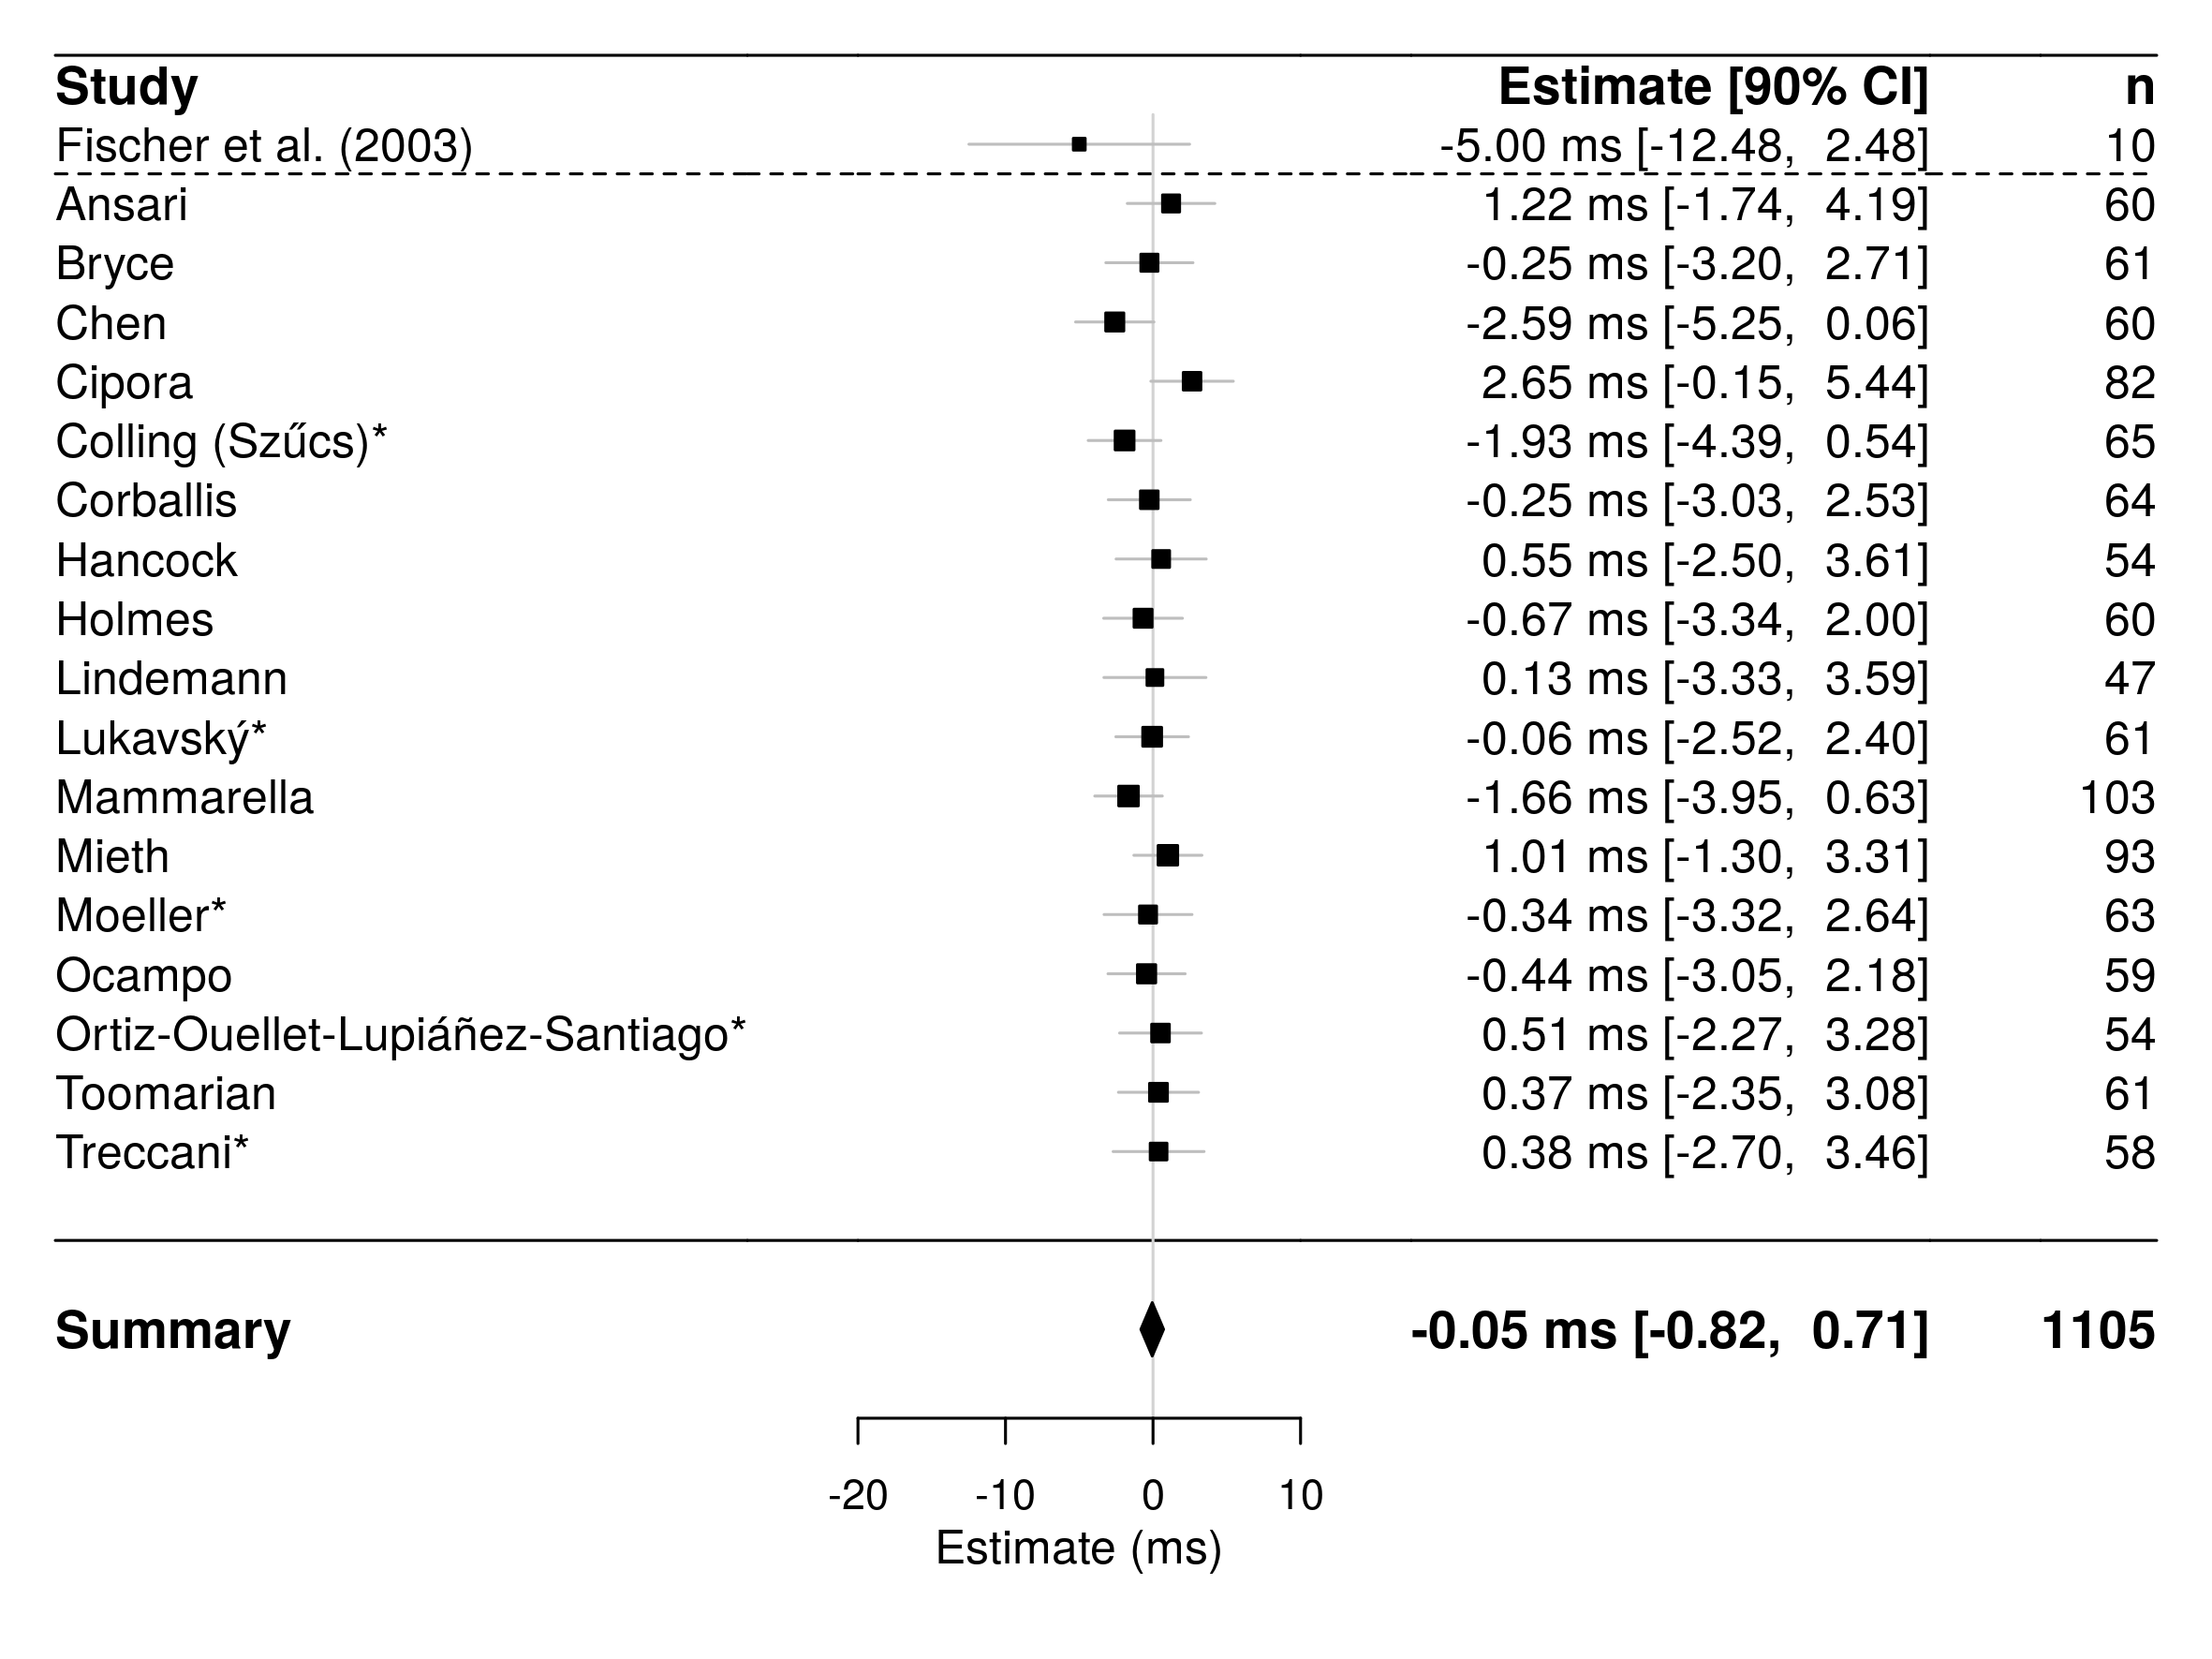
\includegraphics[]{d250}
        \caption{250 ms ISI Condition}
    \end{subfigure}
    \begin{subfigure}{.5\textwidth}
        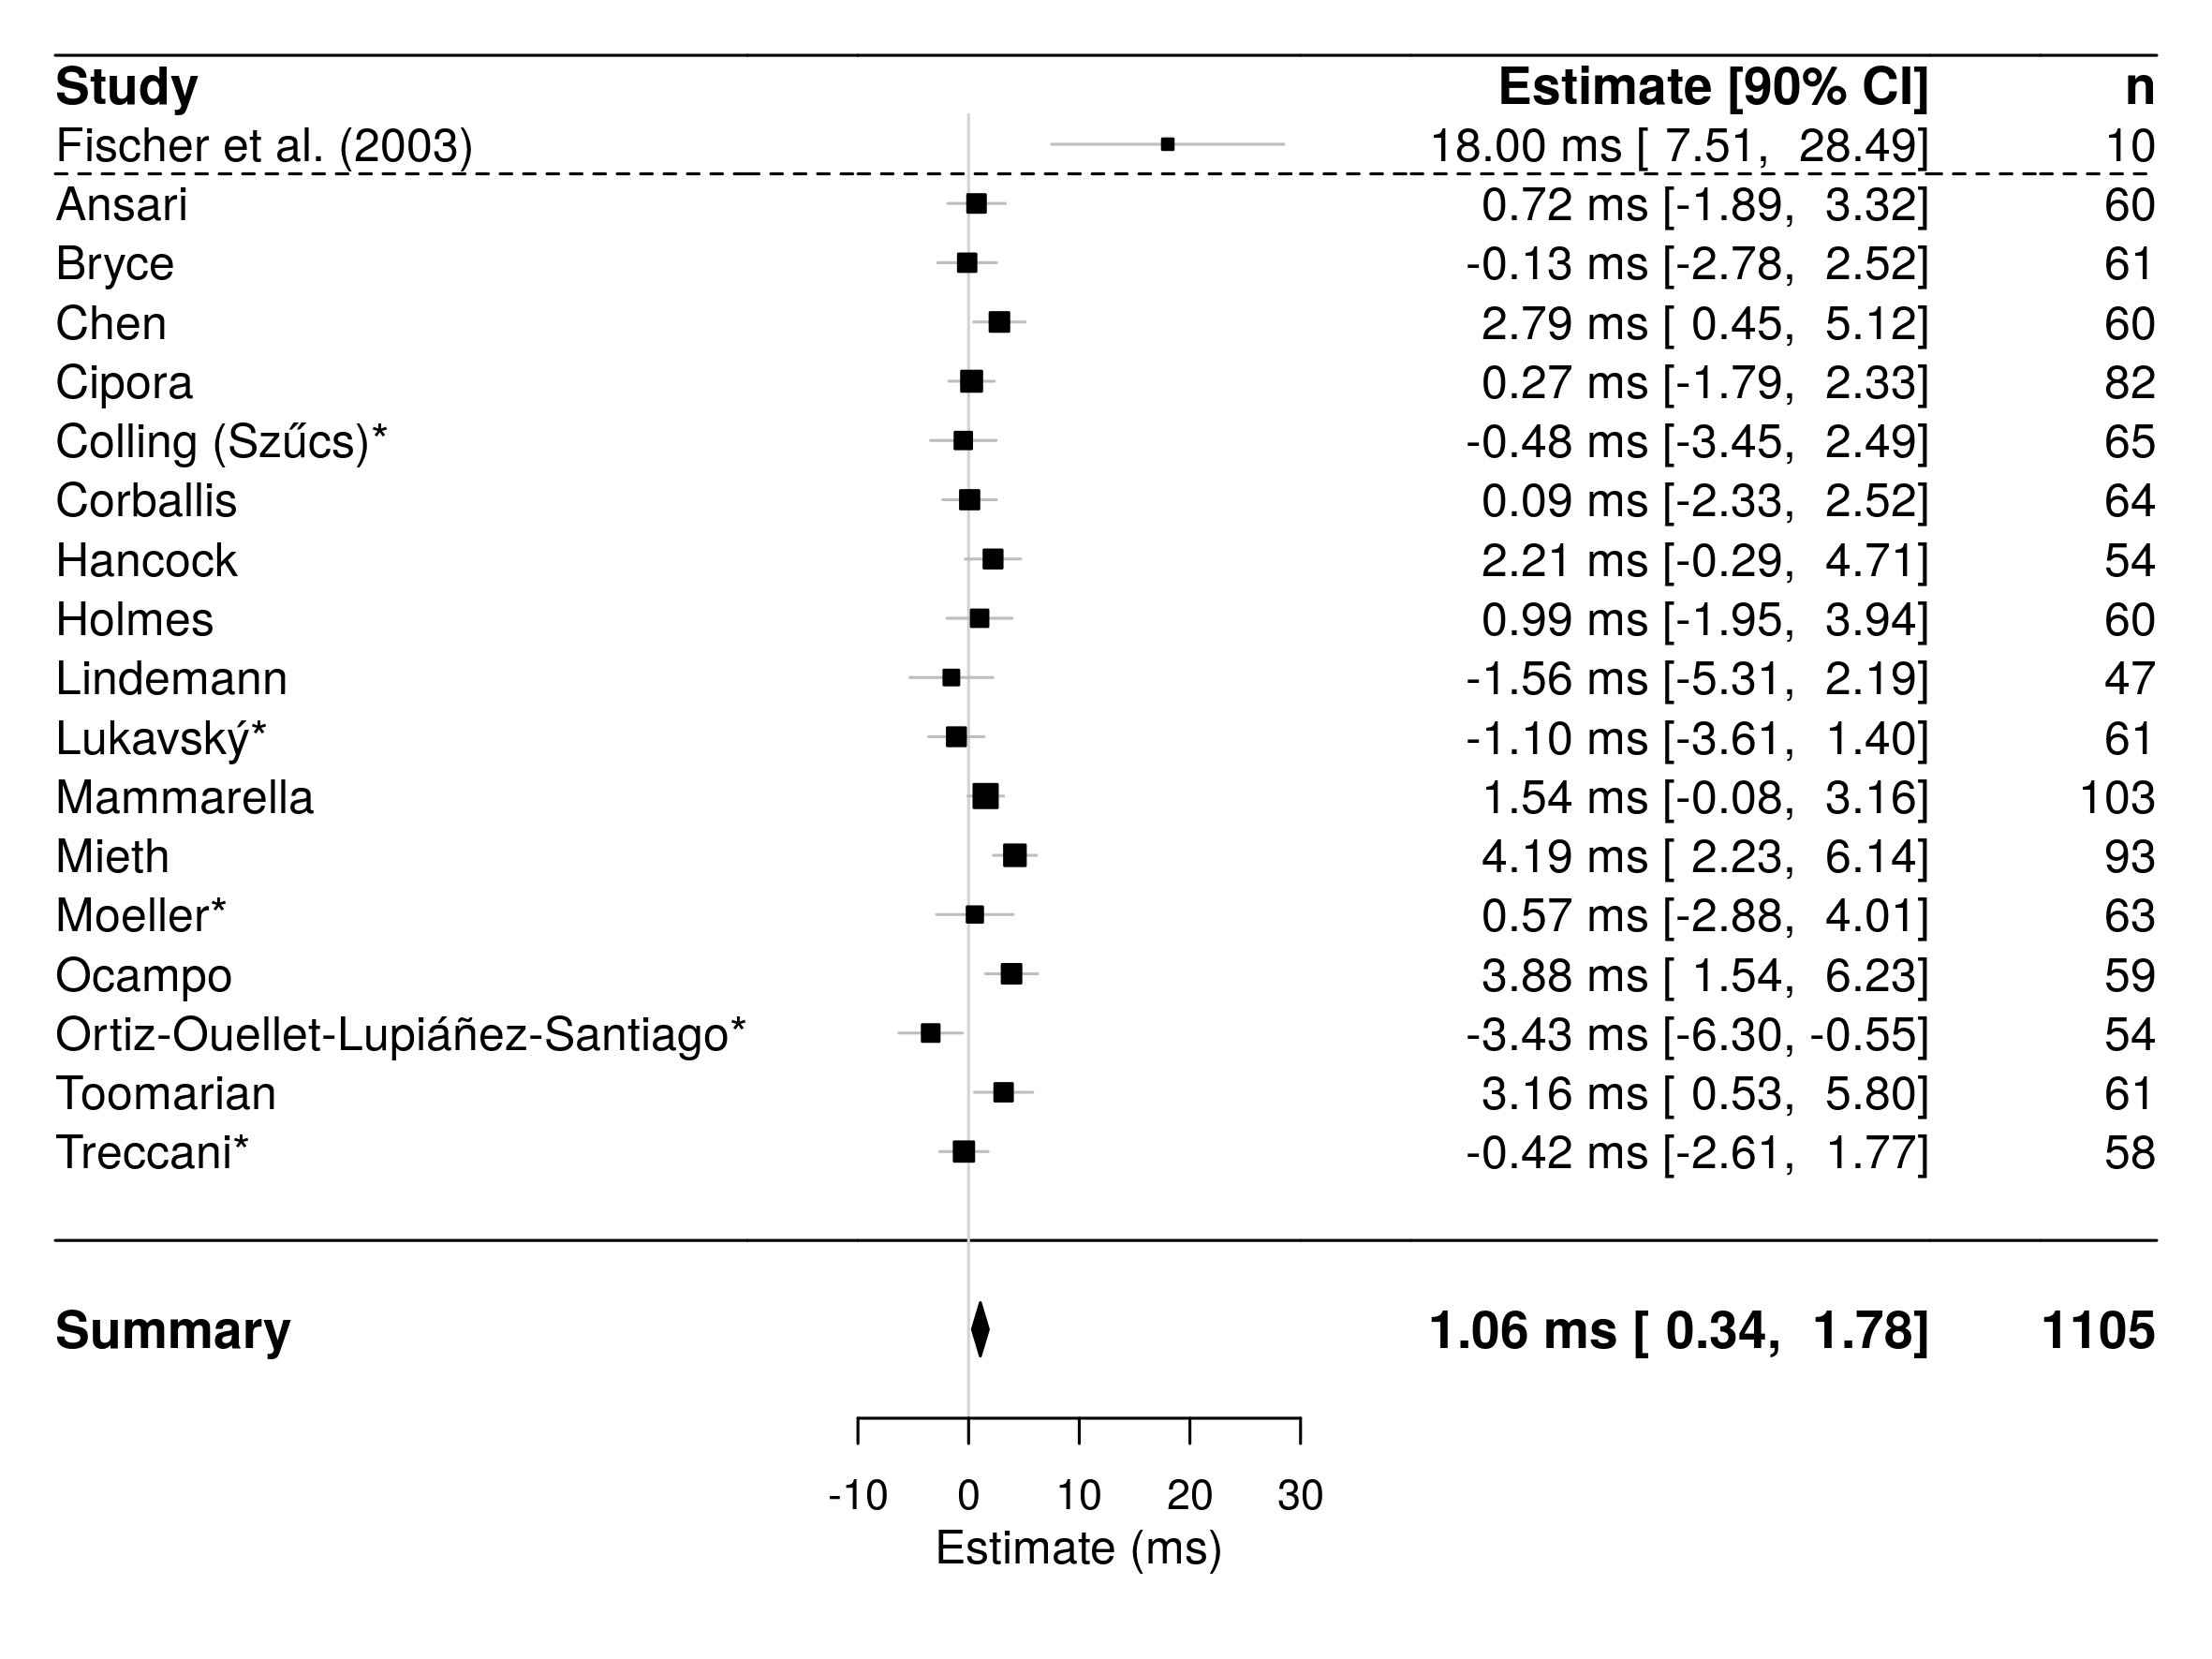
\includegraphics[]{d500}
        \caption{500 ms ISI Condition}
    \end{subfigure}
\end{figure}\begin{figure}[H]
    \centering
    \ContinuedFloat % continue from previous page
    \begin{subfigure}{.5\textwidth}
        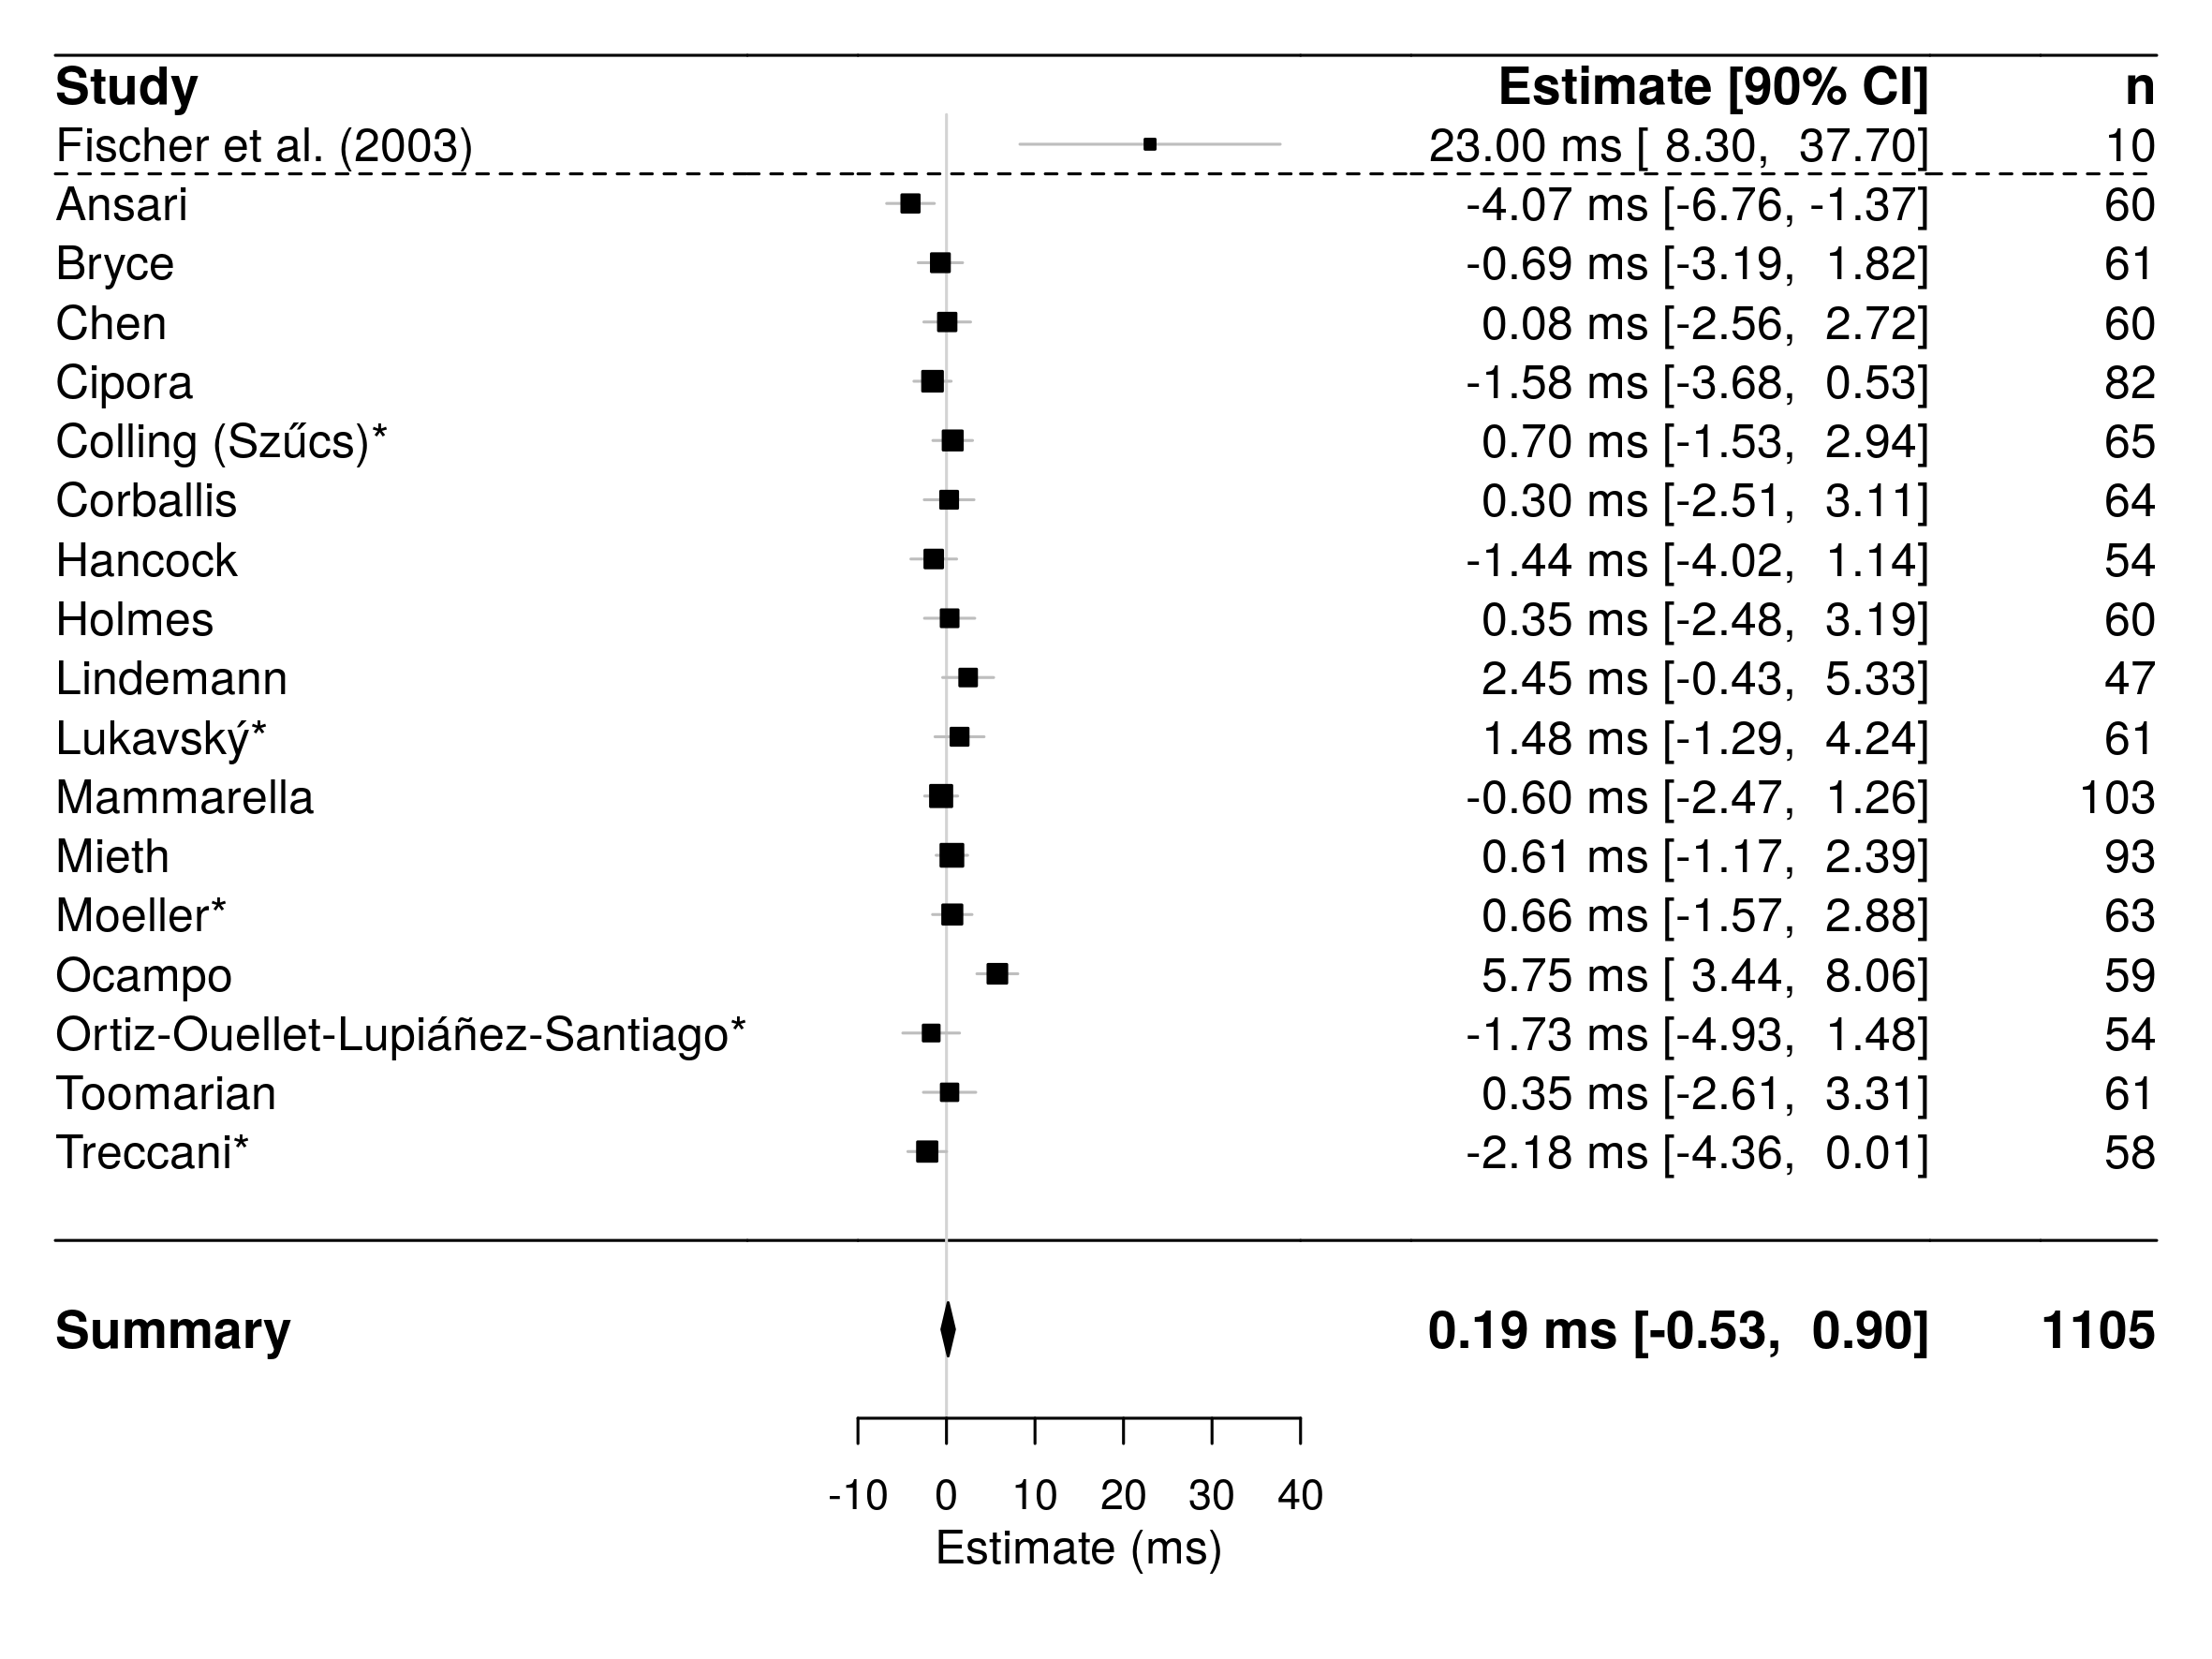
\includegraphics[]{d750}
        \caption{750 ms ISI Condition}
    \end{subfigure}
    \begin{subfigure}{.5\textwidth}
        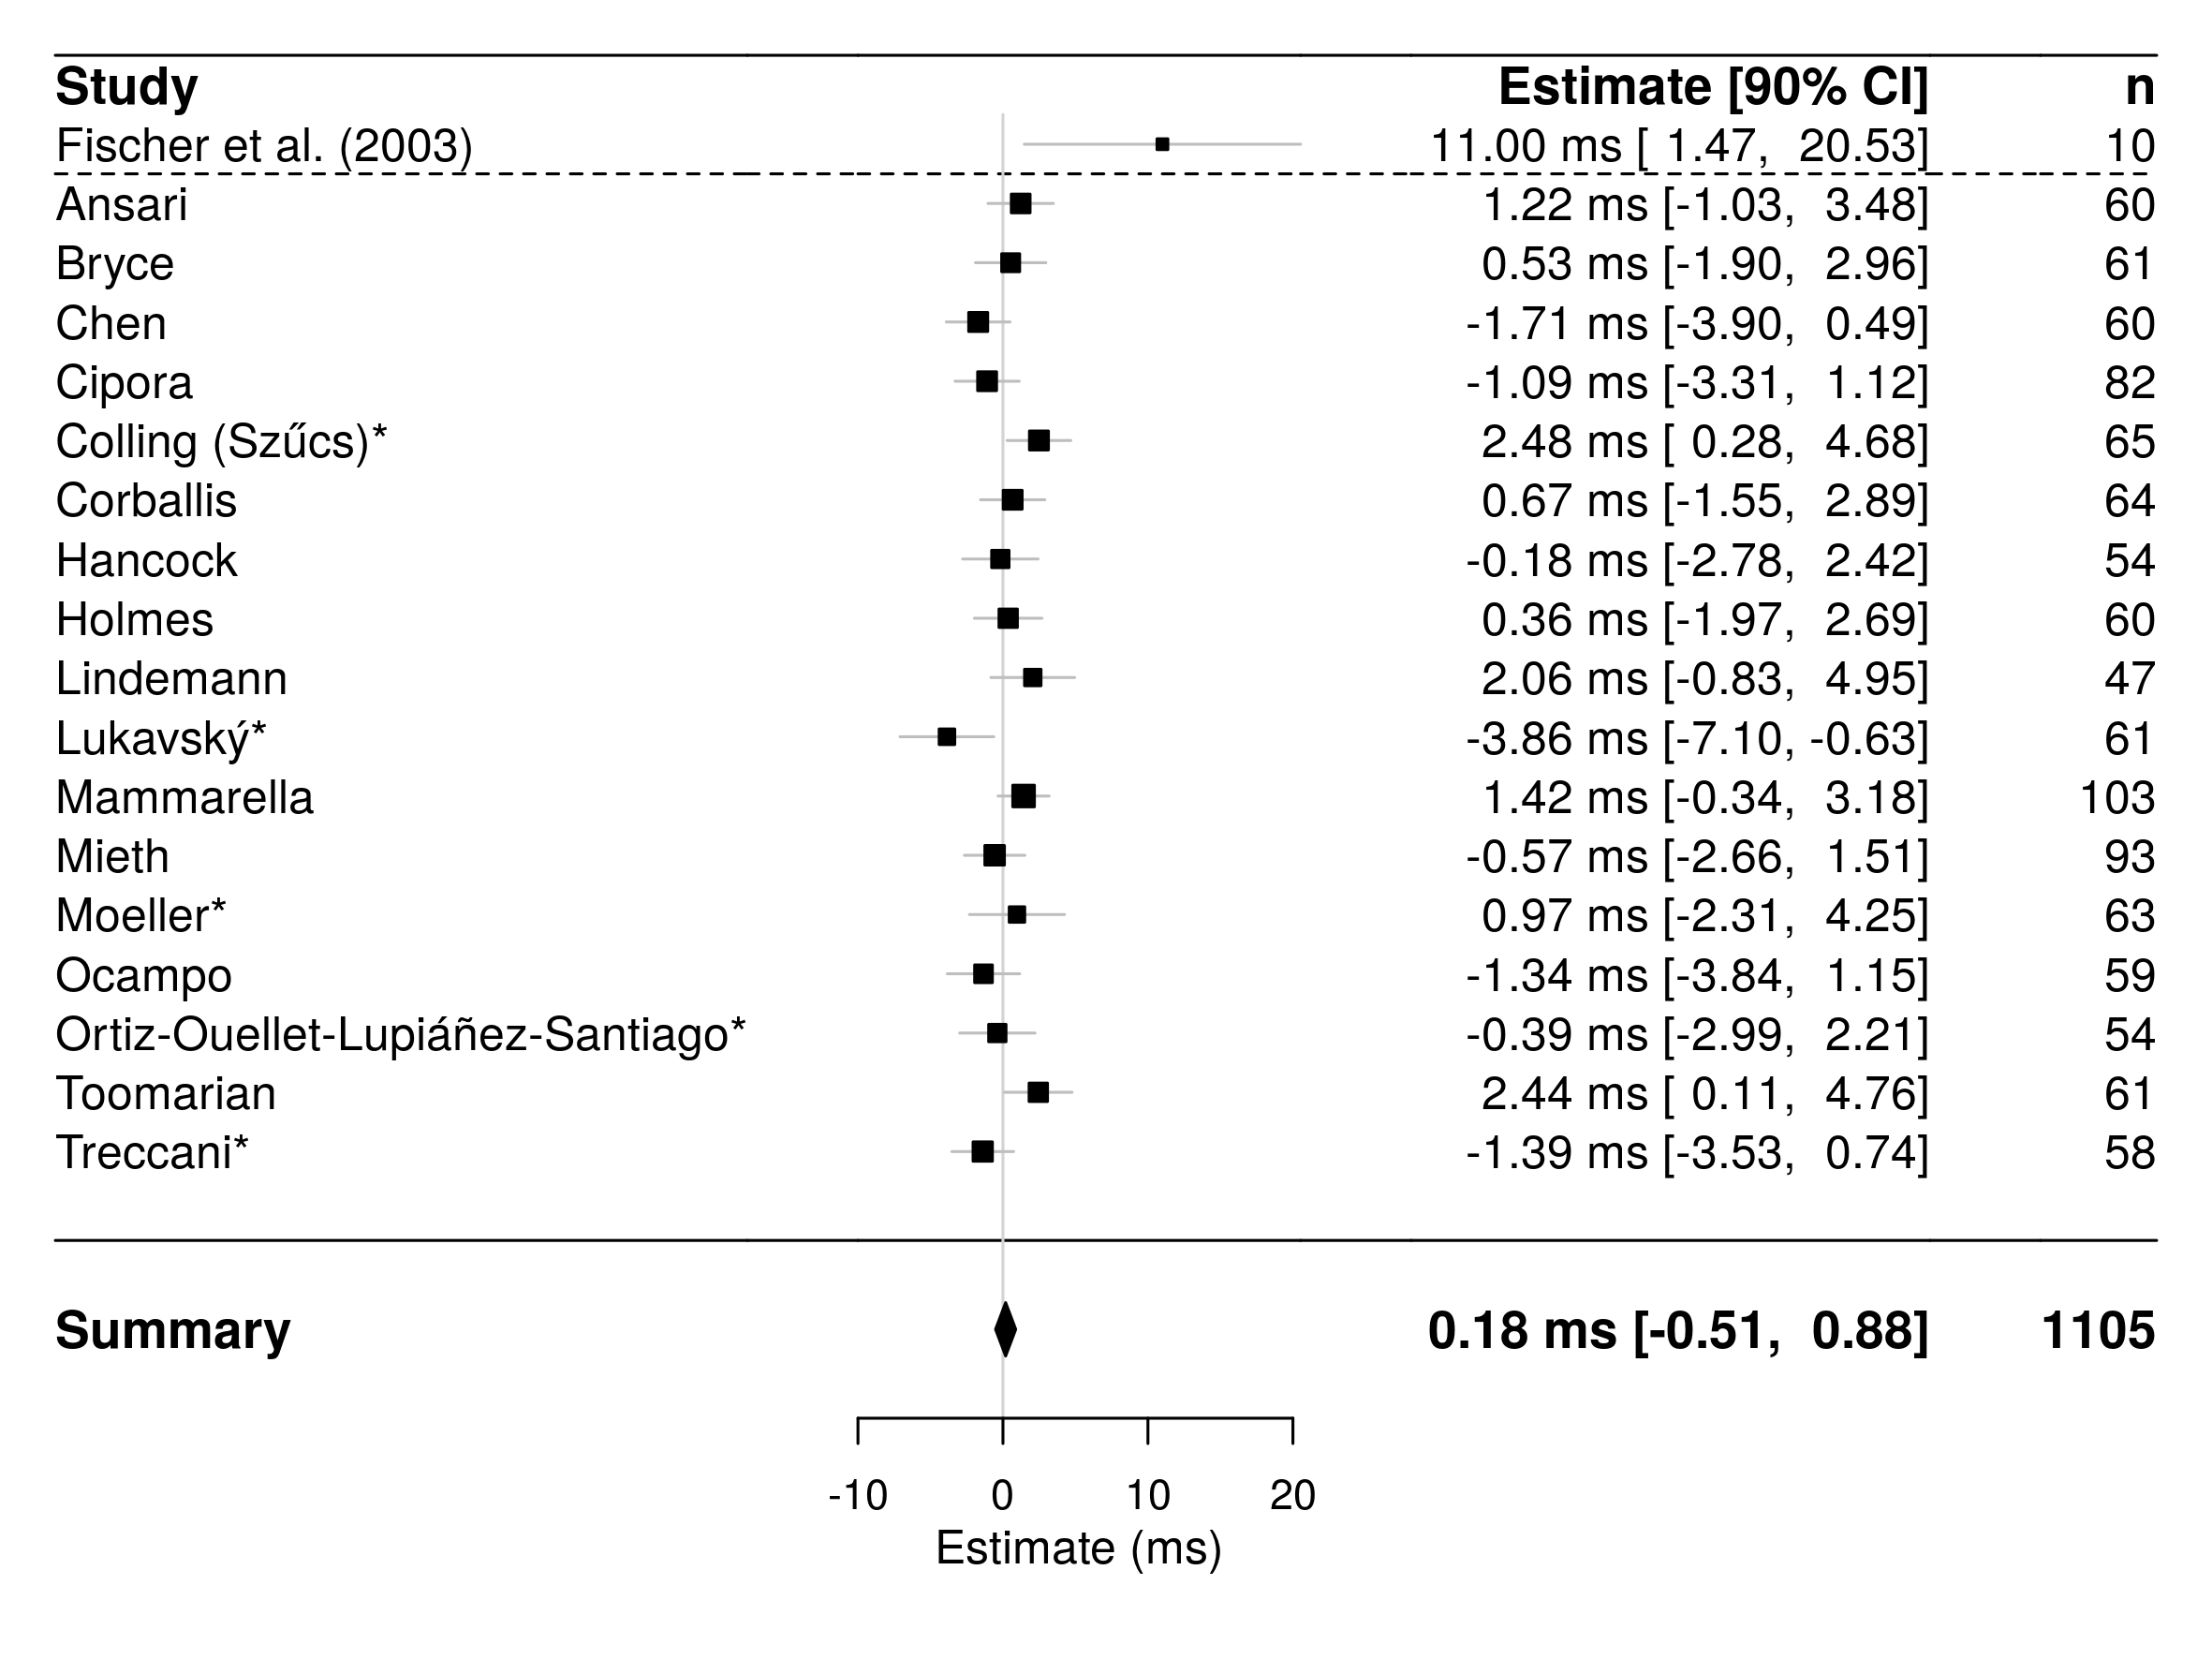
\includegraphics[]{d1000}
        \caption{1000 ms ISI Condition}
    \end{subfigure}
    \caption{Summary of results from Experiment 2 of Fischer, Castel, Dodd, and Pratt (2003), each lab in the present study, and Model 1. Each panel presents the estimate for a given interstimulus-interval (ISI) condition: (a) 250 ms, (b) 500 ms, (c) 750 ms, and (d) 1000 ms. The squares give the effect observed in each lab in each ISI condition; the size of each square is inversely proportional to the sample size. The horizontal lines give the 90\% confidence interval (CI) in each lab in each ISI condition, and the diamond gives the Model 1 estimate and 90\% CI. Labs are identified by the last name of their first authors (as listed in the appendix); labs that used an eye tracker are marked with an asterisk. The effects observed both within and across labs were minuscule and incompatible with those observed by Fischer et al. (2003). They were also highly consistent both across ISI conditions and across labs; the latter result suggests that lab-level moderators are unlikely to have driven our results.}\label{fig:model1}
\end{figure}

\subsubsection{Model 2: Finger
counting}\label{model-2-finger-counting-1}

\begin{figure}

{\centering 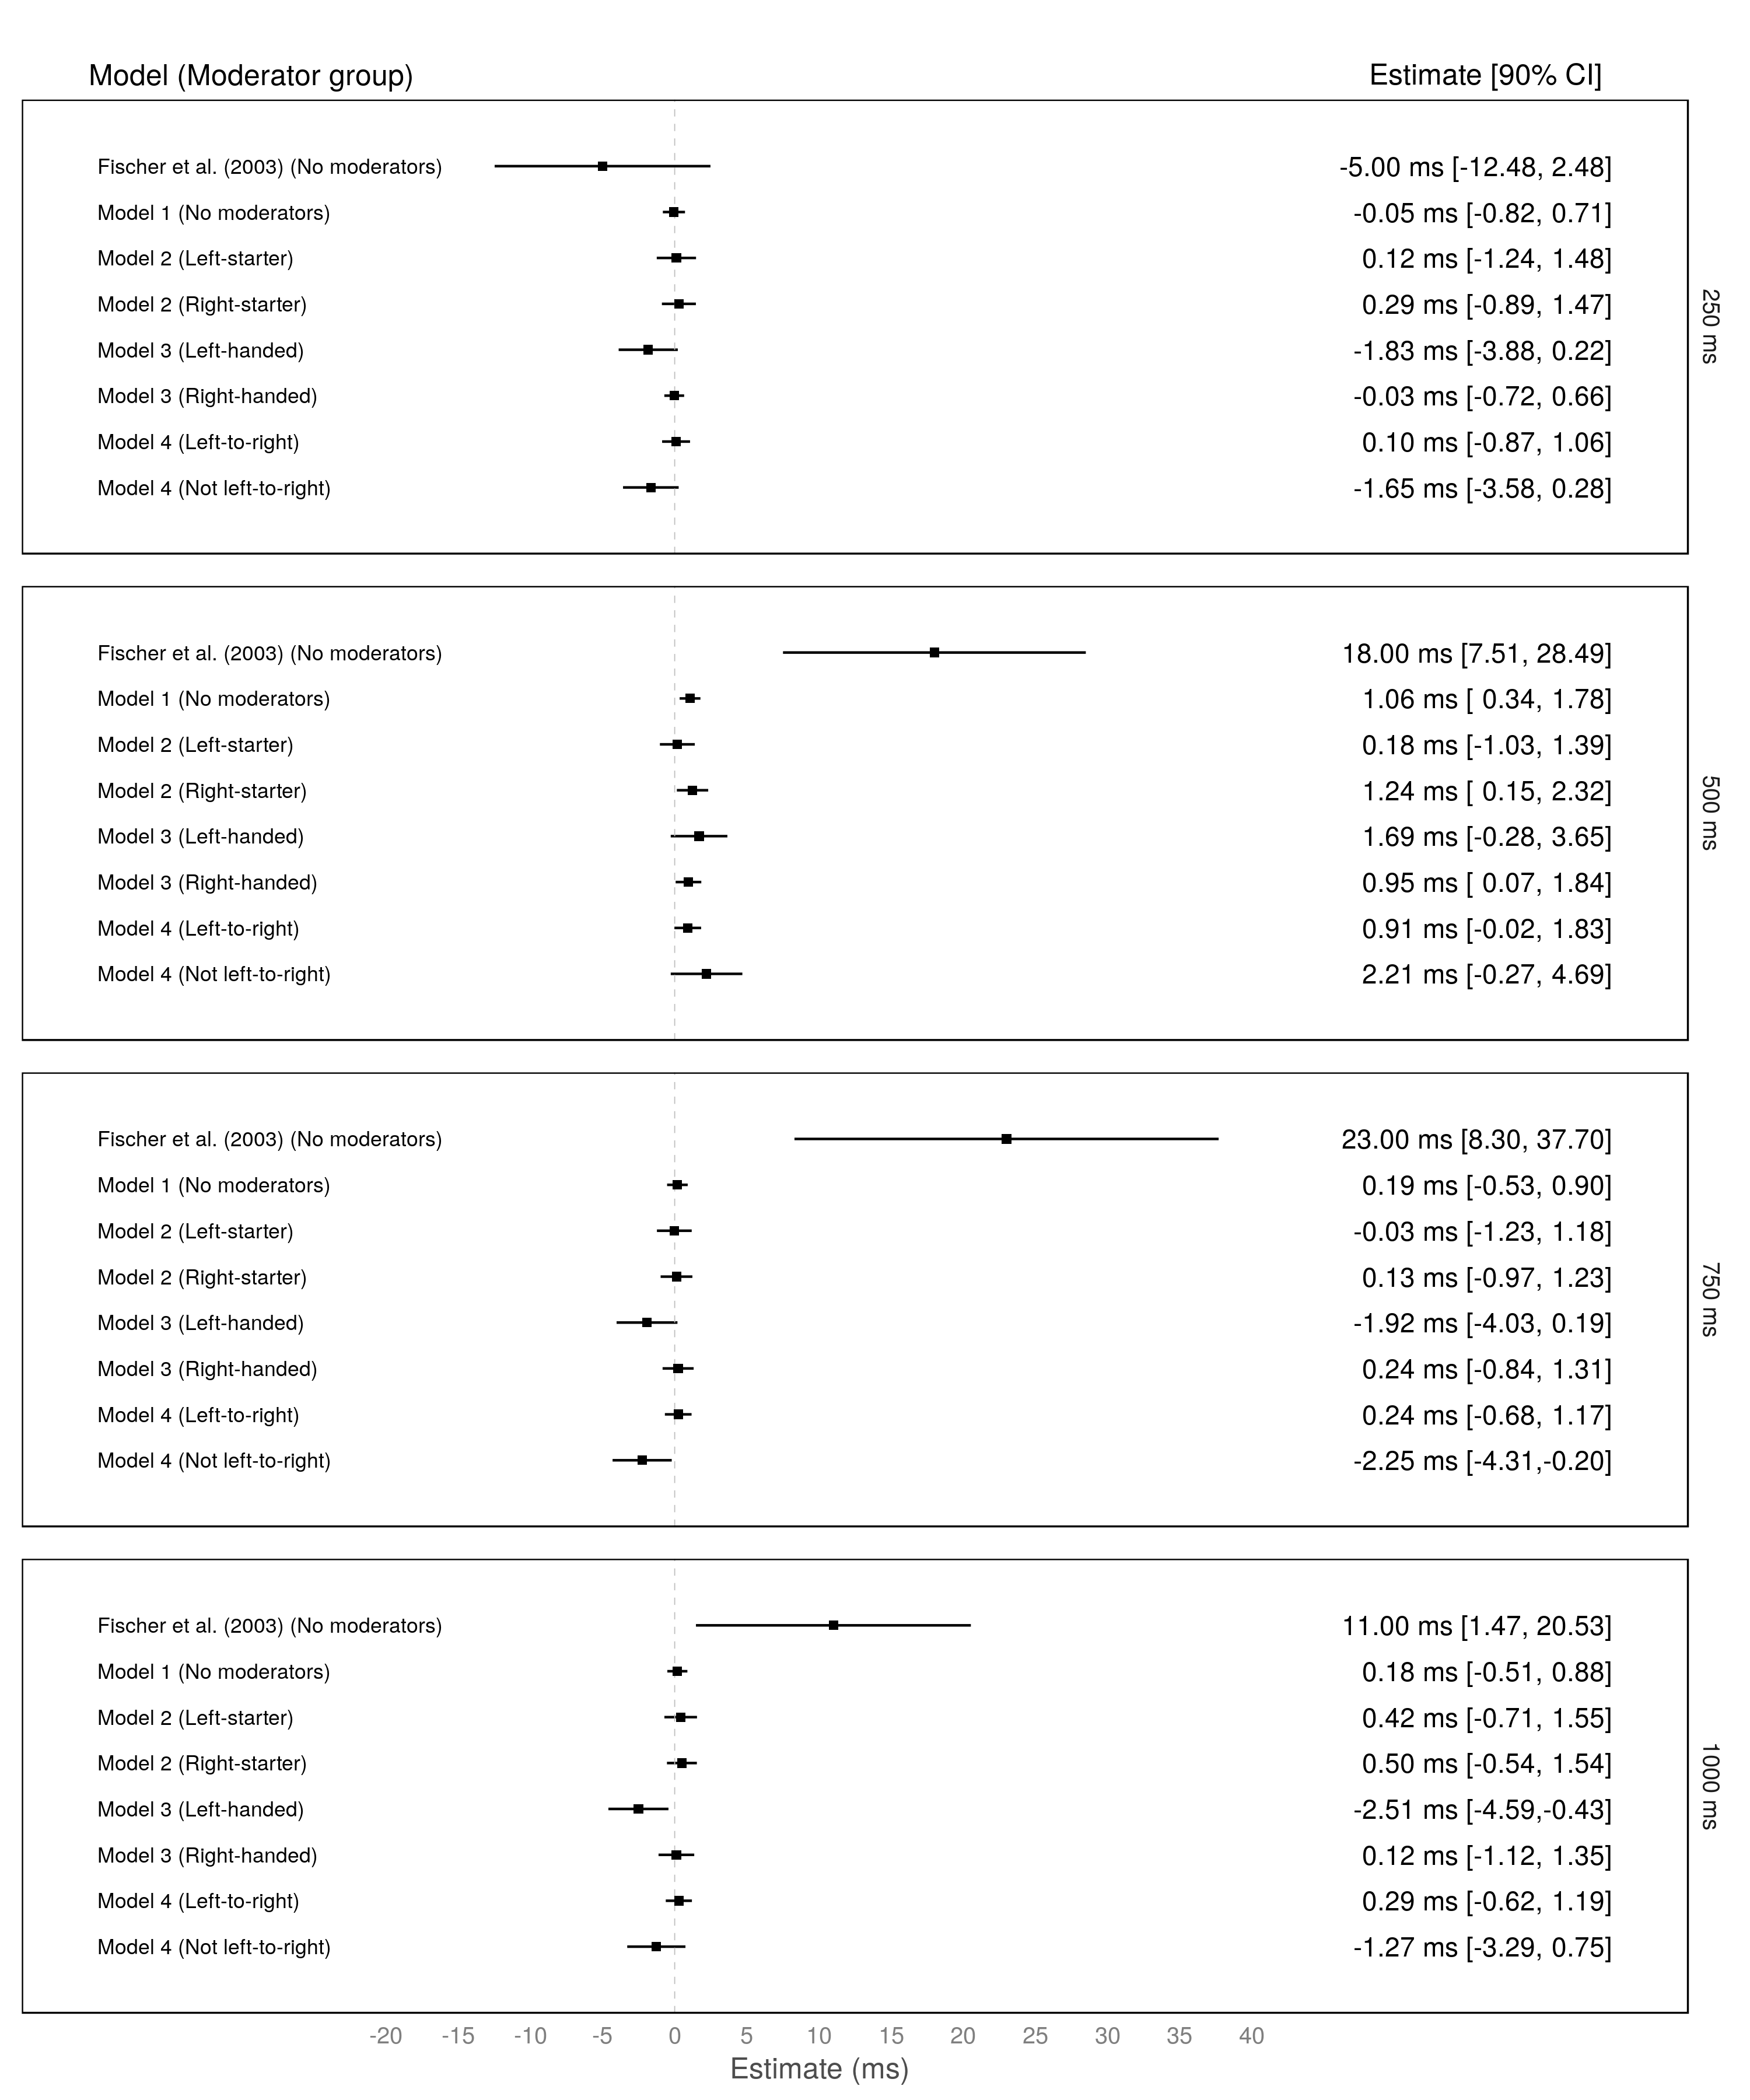
\includegraphics[width=.8\textwidth]{meta_summaryv4} 

}

\caption{Summary of results from Experiment 2 of Fischer, Castel,
Dodd, and Pratt (2003) and Models 1 through 4. Each panel presents the
estimates for a given interstimulus-interval condition: from top to
bottom, 250 ms, 500 ms, 750 ms, and 1000 ms. The squares give the point
estimates, and the horizontal lines give 90\% confidence intervals
(CIs). The effects observed both within and across labs were minuscule
and incompatible with those observed by Fischer et al. (2003). They were
also highly consistent across ISI conditions.}\label{fig:metasum}
\end{figure}

Model 2 was estimated on data from 343 consistent left-starters from 17
labs and 482 consistent right-starters from 17 labs. We summarize the
results from Experiment 2 of \textcite{Fischer:2003ju} along with
results from Models 1 through 4 in Figure \ref{fig:metasum}. Although
previous work suggests a stronger congruency effect among left-starters
and a weaker or possibly even reversed effect among right-starters,
Figure \ref{fig:metasum} shows that finger counting had no substantial
impact on the results. Specifically, the figure shows a minuscule
congruency effect for each finger-counting group in each ISI condition
and minuscule differences between congruency effects for the two
finger-counting groups in each ISI condition (see Tables \ref{tab:count}
and \ref{tab:mod2} in the Supplemental Material for details).










\subsubsection{Model 3: Reading/writing
direction}\label{model-3-readingwriting-direction-1}

Model 3 was estimated on data from 1014 exclusively left-to-right
readers-writers from 17 labs and 76 not exclusively left-to-right
readers-writers from 8 labs. Although previous work suggests a weaker or
possibly even reversed congruency effect among participants who have
experience with languages that are not read and written exclusively from
left to right. Figure \ref{fig:metasum} shows that reading and writing
direction had no substantial impact on the results. Specifically, the
figure shows a minuscule effect for each reading-and-writing-direction
group in each ISI condition and minuscule differences between the
congruency effects for the two reading-and-writing direction groups in
each ISI condition (see Tables \ref{tab:read} and \ref{tab:mod3} in the
Supplemental Material for details).

\subsubsection{Model 4: Handedness}\label{model-4-handedness-1}

Model 4 was estimated on data from 69 left-handed participants from 9
labs and 1007 right-handed participants from 17 labs. Figure
\ref{fig:metasum} shows that handedness had no substantial impact on the
results. Specifically, the figure shows a minuscule effect for each
handedness group in each ISI condition and minuscule differences between
the congruency effects for the two handedness groups in each ISI
condition (see Tables \ref{tab:hand} and \ref{tab:mod4} in the
Supplemental Material for details).

\subsubsection{Model 5: Mathematics fluency and mathematics
anxiety}\label{model-5-mathematics-fluency-and-mathematics-anxiety-1}

Model 5 was estimated on data from 1105 participants from 17 labs.
Although previous work suggests that mathematics fluency and mathematics
anxiety might moderate congruency effects, we observed no substantial
moderating effects (see Table \ref{tab:mod5} in the Supplemental
Material for details).

\subsection{Secondary analyses}\label{secondary-analyses-1}

Model 1 was estimated separately on data from 41 participants (from four
labs) who correctly guessed the purpose of the experiment and also
separately on data from 10468 eye-movement-contaminated trials of 132
participants (from five labs) with contaminated trials in every
combination of ISI and congruency condition. These analyses yielded no
results of substantive interest (see the Supplemental Material for
details).

\section{Discussion}\label{discussion}

The Att-SNARC effect has been used to argue for an early,
response-independent, and automatic origin of the SNARC effect. If the
SNARC effect is produced by early mechanisms, this would provide good
evidence for embodied number representations and support strong claims
about the link between number and space (e.g., a mental number line).

We attempted to replicate Experiment 2 of \textcite{Fischer:2003ju} by
collecting data from 1105 participants at 17 labs. Across these 1105
participants and four ISI conditions, the proportion of times the
congruency effect we observed was positive was .50. Further, the effects
we observed both within and across labs were minuscule and incompatible
with those observed by Fischer et al. Given this, we conclude that we
failed to replicate the effect reported by Fischer et al.

The effects we observed were highly consistent both across ISI
conditions and across labs; the latter result suggests that lab-level
moderators are unlikely to have driven our results. In addition, our
analyses of several participant-level moderators (finger-counting
habits, reading and writing direction, handedness, and mathematics
fluency and mathematics anxiety) revealed no substantial moderating
effects.

We conclude with two important points. First, on the basis of the common
definition of replication employed in practice, one might object that we
did in fact successfully replicate \textcite{Fischer:2003ju}, at least
in the 500-ms ISI condition. In response, we argue that this objection
illustrates one major flaw of that definition: Our result in the 500-ms
ISI condition is manifestly incompatible with the analogous result of
\textcite{Fischer:2003ju}. In addition, we view a difference of about 1
ms, even if \enquote{real,} as too small for any neurally or
psychologically plausible mechanism---particularly one constrained to
operate only within a narrow time window of 500 ms after the stimulus.
That said, we recognize that some such mechanism could be subject to an
arbitrarily large attenuation factor in any particular experimental
paradigm, such as that of Fischer et al., and that potential new
paradigms could reveal an effect. Nonetheless, even if such paradigms
are forthcoming, we maintain on the basis of our results that the
paradigm of Fischer et al. provides no evidence of such a mechanism.

Second, we note several limitations of the present study. First and
foremost, although our results demonstrate that the Att-SNARC effect
cannot be used as evidence to support the strong claims about the link
between number and space discussed earlier, our results do not refute
such accounts. Specifically, although one might, on the basis of our
results, prefer accounts of the SNARC effect that do not imply a mental
number line, the evidence for and against different claims about the
SNARC effect must be viewed in its entirety. The Att-SNARC effect
provides only one such piece of evidence---albeit a particularly strong
and valuable one.

In addition, a set of limitations relates to our sample of participants.
Our sample was recruited primarily from North America, Europe, and
Australasia. Consequently, participants who read and wrote exclusively
from left to right are overrepresented in our data. As reading and
writing direction has been shown to strongly moderate spatial-numerical
associations, it would have been preferable to have more participants
with experience with languages that are not read and written exclusively
from left to right. In addition, data sparsity precluded considering all
moderators jointly in a single model, and thus we considered each
moderator separately.

Finally, the finger-counting assessment we employed did not contain an
explicit instruction to engage in finger counting. As a result, some
participants employed finger counting inconsistently, and they were
therefore excluded from the Model 2 analysis.

\section{Acknowledgements}\label{acknowledgements}

LJC and DS are funded by James S. McDonnell Foundation 21st Century
Science Initiative in Understanding Human Cognition (grant number
220020370; received by DS). We acknowledge the help of the original
authors, in particular Martin Fischer and Jay Pratt. We also note this
project would not have been possible without editor Alex Holcombe's
patient and thoughtful help at every step of the process.

\section{Author contributions}\label{author-contributions}

L. J. Colling and D. Szűcs proposed the study. L. J. Colling programmed
the experiments. L. J. Colling and B. B. McShane developed the analysis
plan and conducted the analyses. L. J. Colling wrote an initial
manuscript. L. J . Colling and B. B. McShane wrote revised and final
manuscripts. All authors critically reviewed the manuscript by providing
comments, feedback, and edits at all stages of writing, and all authors
approved the final manuscript. All authors were involved in data
collection. Authors from the contributing labs provided translated
materials where required (see the appendix).

\printbibliography[title=References]

\clearpage
\makeatletter
\efloat@restorefloats
\makeatother


\begin{appendix}
\section{}
\renewcommand{\thetable}{S\arabic{table}}
\renewcommand{\thefigure}{S\arabic{figure}}

%\pagenumbering{arabic}

\subsection{Primary analyses}\label{primary-analyses}

\subsubsection{Model 1: No Moderators}\label{model-1-no-moderators}

Model 1 was estimated on data from 1105 participants from seventeen labs
(see Table \ref{tab:Exclusions} for details). Of the six equal
allocation multilevel multivariate compound symmetry (EAMMCS) model
specifications, the \emph{Equal Variance, Zero Correlation}
specification was chosen by AIC. AIC; fixed effect estimates, standard
errors, and \(z\)-statistics; and variance component estimates are shown
in Supplementary Table \ref{tab:mod1}.

\subsubsection{Model 2: Finger counting}\label{model-2-finger-counting}

Model 2 was estimated on data from 343 consistent left-starters from
seventeen labs and 482 consistent right-starters from seventeen labs
(see Supplementary Table \ref{tab:count} for details). Of the six EAMMCS
model specifications, the \emph{Equal Variance, Zero Correlation}
specification was chosen by AIC. AIC; fixed effect estimates, standard
errors, and \(z\)-statistics; and variance component estimates are shown
in Supplementary Table \ref{tab:mod2}.

\subsubsection{Model 3: Reading/writing
direction}\label{model-3-readingwriting-direction}

Model 3 was estimated on data from 1014 exclusively left-to-right
readers/writers from seventeen labs and 76 not exclusively left-to-right
readers/writers from eight labs (see Supplementary Table \ref{tab:read}
for details). Of the six EAMMCS model specifications, the \emph{Equal
Variance, Zero Correlation} specification was chosen by AIC. AIC; fixed
effect estimates, standard errors, and \(z\)-statistics; and variance
component estimates are shown in Supplementary Table \ref{tab:mod3}.

\subsubsection{Model 4: Handedness}\label{model-4-handedness}

Model 4 was estimated on data from 69 left-handed participants from nine
labs and 1007 right-handed participants from seventeen labs (see
Supplementary Table \ref{tab:hand} for details). Of the six EAMMCS model
specifications, the \emph{Unequal Variance, Zero Correlation}
specification was chosen by AIC. AIC; fixed effect estimates, standard
errors, and \(z\)-statistics; and variance component estimates are shown
in Supplementary Table \ref{tab:mod4}.

\subsubsection{Model 5: Mathematics fluency and mathematics
anxiety}\label{model-5-mathematics-fluency-and-mathematics-anxiety}

Model 5 was estimated on data from 1105 participants from seventeen labs
(see Table \ref{tab:Exclusions}). See the main text for model
specification details, but note that (i) for consistency with Model 1 we
employed the \emph{Equal Variance, Zero Correlation} specification for
effects for each ISI condition for each lab and (ii) the math test and
AMAS were centred and scaled by their respective means and standard
deviations across the 1105 participants prior to estimation of the
model. Fixed effect estimates, standard errors, and \(t\)-statistics and
variance component estimates are shown in Supplementary Table
\ref{tab:mod5}.

\subsection{Secondary analyses}\label{secondary-analyses}

\subsubsection{Purpose of experiment}\label{purpose-of-experiment}

Data from several participants were not included in the primary analysis
because they correctly guessed the purpose of the experiment (as
assessed by the exit questionnaire). The data from these participants
was analyzed separately to determine whether insight into the purpose of
the experiment moderated the effect. Specifically, Model 1 was estimated
on data from the 41 participants from four labs who correctly guessed
the purpose of the experiment (see Supplementary Table \ref{tab:mod1bn}
for details). Of the six model EAMMCS model specifications, the
\emph{Equal Variance, Zero Correlation} specification was chosen by AIC.
AIC; fixed effect estimates, standard errors, and \(z\)-statistics; and
variance component estimates are shown in Supplementary Table
\ref{tab:mod1b}.

\subsubsection{Eye-movement contaminated
trials}\label{eye-movement-contaminated-trials}

Data from individual trials that were contaminated with eye movements
were also not included the primary analysis. The data from these trials
was analyzed separately to determine whether eye movements moderated the
effect. Specifically, Model 1 was estimated on data from 10468 eye
movement contaminated trials of 132 participants from five labs with
contaminated trials in every combination of ISI and congruency
congruency condition (see Supplementary Table \ref{tab:Eyedetail} for
details). Of the six EAMMCS model specifications, the \emph{Fixed
Effects} specification was chosen by AIC. AIC; fixed effect estimates,
standard errors, and \(z\)-statistics; and variance component estimates
are shown in Supplementary Table \ref{tab:mod1c}

\begin{table}[!p]
\caption{\label{tab:mod1}Model 1 Estimates.}
\begin{subtable}{\textwidth}
\subcaption{AIC}
\centering
\begin{table}[H]\centering\begingroup\fontsize{10}{12}\selectfont

\begin{tabular}{lr}
\toprule
Specification & AIC\\
\midrule
Fixed Effects & 264.12\\
Equal Variance, Zero Correlation & 259.66\\
Equal Variance, Single Correlation & 261.64\\
Unequal Variance, Zero Correlation & 261.04\\
Unequal Variance, Single Correlation & 260.87\\
No Constraints & 270.83\\
\bottomrule
\end{tabular}\endgroup{}
\end{table}
\end{subtable}
\begin{subtable}{\textwidth}
\caption{Fixed Effect Estimates}
\centering
\begin{table}[H]\centering\begingroup\fontsize{10}{12}\selectfont

\begin{tabular}{lrrr}
\toprule
ISI Condition & Estimate & Std. Err. & $z$\\
\midrule
250  ms & -0.05 & 0.47 & -0.11\\
500  ms & 1.06 & 0.44 & 2.43\\
750  ms & 0.19 & 0.43 & 0.43\\
1000 ms & 0.18 & 0.42 & 0.44\\
\bottomrule
\end{tabular}\endgroup{}
\end{table}
\end{subtable}
\begin{subtable}{\textwidth}
\caption{Variance Component Estimates. Estimates are presented on the standard deviation scale. }
\centering
\begin{table}[H]\centering\begingroup\fontsize{10}{12}\selectfont

\begin{tabular}{lr}
\toprule
ISI Condition & Estimate\\
\midrule
250 ms & 1.02\\
500 ms & 1.02\\
750 ms & 1.02\\
1000 ms & 1.02\\
\bottomrule
\end{tabular}\endgroup{}
\end{table}
\end{subtable}
\end{table}

\begin{table}

\caption{\label{tab:count}Number of participants in each finger counting group for each of the seventeen labs.}
\centering
\begin{tabular}[t]{lccccc}
\toprule
Lab & \makecell[c]{Consistent\\Left-starter} & \makecell[c]{Inconsistent\\Left-starter} & \makecell[c]{No\\Group} & \makecell[c]{Inconsistent\\Right-starter} & \makecell[c]{Consistent\\Right-starter}\\
\midrule
Ansari & 23 & 2 & 2 & 3 & 30\\
Bryce & 13 & 8 & 2 & 17 & 21\\
Chen & 22 & 0 & 2 & 0 & 36\\
Cipora & 19 & 9 & 5 & 18 & 31\\
Colling (Szűcs) & 21 & 3 & 11 & 3 & 27\\
Corballis & 18 & 3 & 5 & 4 & 34\\
Hancock & 22 & 6 & 0 & 3 & 23\\
Holmes & 14 & 2 & 1 & 8 & 35\\
Lindemann & 22 & 1 & 4 & 1 & 19\\
Lukavský & 12 & 7 & 2 & 16 & 24\\
Mammarella & 30 & 8 & 6 & 23 & 36\\
Mieth & 32 & 10 & 10 & 16 & 25\\
Moeller & 23 & 0 & 6 & 0 & 34\\
Ocampo & 27 & 0 & 2 & 0 & 30\\
Ortiz-Ouellet-Lupiáñez-Santiago & 10 & 8 & 4 & 22 & 10\\
Toomarian & 19 & 0 & 0 & 0 & 42\\
Treccani & 16 & 7 & 4 & 6 & 25\\
\bottomrule
\end{tabular}
\end{table}

\begin{table}[!p]
\caption{\label{tab:mod2}Model 2 Estimates.}
\begin{subtable}{\textwidth}
\subcaption{AIC}
\centering
\begin{table}[H]\centering\begingroup\fontsize{10}{12}\selectfont

\begin{tabular}{lr}
\toprule
Specification & AIC\\
\midrule
Fixed Effects & 665.97\\
Equal Variance, Zero Correlation & 637.31\\
Equal Variance, Single Correlation & 639.00\\
Unequal Variance, Zero Correlation & 638.57\\
Unequal Variance, Single Correlation & 640.13\\
No Constraints & 646.51\\
\bottomrule
\end{tabular}\endgroup{}
\end{table}
\end{subtable}
\begin{subtable}{\textwidth}
\caption{Fixed Effect Estimates}
\centering
\begin{table}[H]\centering\begingroup\fontsize{10}{12}\selectfont

\begin{tabular}{llrrr}
\toprule
ISI Condition & Finger counting group & Estimate & Std. Err. & $z$\\
\midrule
250  ms & Consistent Right-starter & 0.29 & 0.72 & 0.40\\
250  ms & Consistent Left-starter & 0.12 & 0.83 & 0.14\\
500  ms & Consistent Right-starter & 1.24 & 0.66 & 1.88\\
500  ms & Consistent Left-starter & 0.18 & 0.74 & 0.24\\
750  ms & Consistent Right-starter & 0.13 & 0.67 & 0.19\\
750  ms & Consistent Left-starter & -0.03 & 0.73 & -0.04\\
1000 ms & Consistent Right-starter & 0.50 & 0.63 & 0.79\\
1000 ms & Consistent Left-starter & 0.42 & 0.69 & 0.61\\
\bottomrule
\end{tabular}\endgroup{}
\end{table}
\end{subtable}
\begin{subtable}{\textwidth}
\caption{Variance Component Estimates. Estimates are presented on the standard deviation scale. 39\% of the variance is estimated to be at the lab-level and 61\% at the group-level.}
\centering
\begin{table}[H]\centering\begingroup\fontsize{10}{12}\selectfont

\begin{tabular}{lr}
\toprule
ISI Condition & Estimate\\
\midrule
250 ms & 1.74\\
500 ms & 1.74\\
750 ms & 1.74\\
1000 ms & 1.74\\
\bottomrule
\end{tabular}\endgroup{}
\end{table}
\end{subtable}
\end{table}

\begin{table}

\caption{\label{tab:read}Number of participants in each of the reading/writing direction groups for each of the seventeen labs.}
\centering
\begin{tabular}[t]{lcc}
\toprule
Lab & \makecell[c]{Exclusively\\Left-to-Right} & \makecell[c]{Not exclusively\\Left-to-Right}\\
\midrule
Ansari & 55 & 5\\
Bryce & 59 & 2\\
Chen & 39 & 21\\
Cipora & 76 & 6\\
Colling (Szűcs) & 55 & 10\\
Corballis & 60 & 4\\
Hancock & 53 & 1\\
Holmes & 54 & 6\\
Lindemann & 47 & 0\\
Lukavský & 58 & 3\\
Mammarella & 103 & 0\\
Mieth & 79 & 14\\
Moeller & 54 & 9\\
Ocampo & 55 & 4\\
Ortiz-Ouellet-Lupiáñez-Santiago & 54 & 0\\
Toomarian & 56 & 5\\
Treccani & 57 & 1\\
\bottomrule
\end{tabular}
\end{table}

\begin{table}[!p]
\caption{\label{tab:mod3}Model 3 Estimates.}
\begin{subtable}{\textwidth}
\subcaption{AIC}
\centering
\begin{table}[H]\centering\begingroup\fontsize{10}{12}\selectfont

\begin{tabular}{lr}
\toprule
Specification & AIC\\
\midrule
Fixed Effects & 495.58\\
Equal Variance, Zero Correlation & 448.05\\
Equal Variance, Single Correlation & 449.41\\
Unequal Variance, Zero Correlation & 451.89\\
Unequal Variance, Single Correlation & 453.44\\
No Constraints & 457.83\\
\bottomrule
\end{tabular}\endgroup{}
\end{table}
\end{subtable}
\begin{subtable}{\textwidth}
\caption{Fixed Effect Estimates}
\centering
\begin{table}[H]\centering\begingroup\fontsize{10}{12}\selectfont

\begin{tabular}{llrrr}
\toprule
ISI Condition &  Reading/Writing Direction & Estimate & Std. Err. & $z$\\
\midrule
250  ms & Exclusively LTR & 0.10 & 0.59 & 0.17\\
250  ms & Not exclusively LTR & -1.65 & 1.17 & -1.41\\
500  ms & Exclusively LTR & 0.91 & 0.56 & 1.62\\
500  ms & Not exclusively LTR & 2.21 & 1.51 & 1.46\\
750  ms & Exclusively LTR & 0.24 & 0.56 & 0.43\\
750  ms & Not exclusively LTR & -2.25 & 1.25 & -1.80\\
1000 ms & Exclusively LTR & 0.29 & 0.55 & 0.53\\
1000 ms & Not exclusively LTR & -1.27 & 1.23 & -1.03\\
\bottomrule
\end{tabular}\endgroup{}
\end{table}
\end{subtable}
\begin{subtable}{\textwidth}
\caption{Variance Component Estimates. Estimates are presented on the standard deviation scale. 10\% of the variance is estimated to be at the lab-level and 90\% at the group-level.}
\centering
\begin{table}[H]\centering\begingroup\fontsize{10}{12}\selectfont

\begin{tabular}{lr}
\toprule
ISI Condition & Estimate\\
\midrule
250 ms & 1.71\\
500 ms & 1.71\\
750 ms & 1.71\\
1000 ms & 1.71\\
\bottomrule
\end{tabular}\endgroup{}
\end{table}
\end{subtable}
\end{table}

\begin{table}

\caption{\label{tab:hand}Number of participants in each handedness group for each of the seventeen labs.}
\centering
\begin{tabular}[t]{lcc}
\toprule
Lab & \makecell[c]{Left-\\handed} & \makecell[c]{Right-\\handed}\\
\midrule
Ansari & 4 & 56\\
Bryce & 4 & 57\\
Chen & 5 & 55\\
Cipora & 3 & 79\\
Colling (Szűcs) & 7 & 58\\
Corballis & 9 & 55\\
Hancock & 6 & 48\\
Holmes & 4 & 56\\
Lindemann & 5 & 42\\
Lukavský & 7 & 54\\
Mammarella & 6 & 97\\
Mieth & 14 & 79\\
Moeller & 4 & 59\\
Ocampo & 4 & 55\\
Ortiz-Ouellet-Lupiáñez-Santiago & 3 & 51\\
Toomarian & 10 & 51\\
Treccani & 3 & 55\\
\bottomrule
\end{tabular}
\end{table}

\begin{table}[!p]
\caption{\label{tab:mod4}Model 4 Estimates.}
\begin{subtable}{\textwidth}
\subcaption{AIC}
\centering
\begin{table}[H]\centering\begingroup\fontsize{10}{12}\selectfont

\begin{tabular}{lr}
\toprule
Specification & AIC\\
\midrule
Fixed Effects & 598.41\\
Equal Variance, Zero Correlation & 473.56\\
Equal Variance, Single Correlation & 475.56\\
Unequal Variance, Zero Correlation & 470.86\\
Unequal Variance, Single Correlation & 472.48\\
No Constraints & 480.12\\
\bottomrule
\end{tabular}\endgroup{}
\end{table}
\end{subtable}
\begin{subtable}{\textwidth}
\caption{Fixed Effect Estimates}
\centering
\begin{table}[H]\centering\begingroup\fontsize{10}{12}\selectfont

\begin{tabular}{llrrr}
\toprule
ISI Condition & Handedness Group & Estimate & Std. Err. & $z$\\
\midrule
250  ms & Right-handed & -0.03 & 0.42 & -0.07\\
250  ms & Left-handed & -1.83 & 1.25 & -1.46\\
500  ms & Right-handed & 0.95 & 0.54 & 1.76\\
500  ms & Left-handed & 1.69 & 1.19 & 1.42\\
750  ms & Right-handed & 0.24 & 0.65 & 0.37\\
750  ms & Left-handed & -1.92 & 1.28 & -1.50\\
1000 ms & Right-handed & 0.12 & 0.75 & 0.16\\
1000 ms & Left-handed & -2.51 & 1.27 & -1.98\\
\bottomrule
\end{tabular}\endgroup{}
\end{table}
\end{subtable}
\begin{subtable}{\textwidth}
\caption{Variance Component Estimates. Estimates are presented on the standard deviation scale. 12\% of the variance is estimated to be at the lab-level and 88\% at the group-level.}
\centering
\begin{table}[H]\centering\begingroup\fontsize{10}{12}\selectfont

\begin{tabular}{lr}
\toprule
ISI Condition & Estimate\\
\midrule
250 ms & 0.01\\
500 ms & 1.57\\
750 ms & 2.19\\
1000 ms & 2.71\\
\bottomrule
\end{tabular}\endgroup{}
\end{table}
\end{subtable}
\end{table}

\begin{table}[!p]
\caption{\label{tab:mod5}Model 5 Estimates.}
\begin{subtable}{\textwidth}
\subcaption{Fixed Effect Estimates}
\centering
\begin{table}[H]\centering\begingroup\fontsize{10}{12}\selectfont

\begin{tabular}{lccc}
\toprule
Effect & Estimate & Std. Err. & $t$\\
\midrule
250 ms ISI & -0.03 & 0.44 & -0.07\\
500 ms ISI & 0.88 & 0.44 & 2.02\\
750 ms ISI & 0.01 & 0.44 & 0.02\\
1000 ms ISI & 0.21 & 0.44 & 0.48\\
250 ms ISI $\times$ Maths test & -0.15 & 0.42 & -0.35\\
500 ms ISI $\times$ Maths test & -0.80 & 0.42 & -1.90\\
750 ms ISI $\times$ Maths test & -0.24 & 0.42 & -0.57\\
1000 ms ISI $\times$ Maths test & 0.08 & 0.42 & 0.18\\
250 ms ISI $\times$ AMAS & -0.66 & 0.40 & -1.66\\
500 ms ISI $\times$ AMAS & 0.29 & 0.40 & 0.73\\
750 ms ISI $\times$ AMAS & -0.21 & 0.40 & -0.54\\
1000 ms ISI $\times$ AMAS & -0.57 & 0.40 & -1.44\\
250 ms ISI $\times$ Maths test $\times$ AMAS & -0.12 & 0.39 & -0.30\\
500 ms ISI $\times$ Maths test $\times$ AMAS & -0.38 & 0.39 & -0.98\\
750 ms ISI $\times$ Maths test $\times$ AMAS & -0.24 & 0.39 & -0.63\\
1000 ms ISI $\times$ Maths test $\times$ AMAS & 0.22 & 0.39 & 0.56\\
\bottomrule
\end{tabular}\endgroup{}
\end{table}
\end{subtable}
\begin{subtable}{\textwidth}
\caption{Variance Component Estimates. Estimates are presented on the standard deviation scale.}
\centering
\begin{table}[H]\centering\begingroup\fontsize{10}{12}\selectfont

\begin{tabular}{lc|lc}
\toprule
ISI Condition & Estimate & Additional Effects & Estimate\\
\midrule
250 ms & 0.85 & Participant & 0.00\\
500 ms & 0.85 & Maths Test & 0.61\\
750 ms & 0.85 & AMAS & 0.33\\
1000 ms & 0.85 & Maths test $\times$ AMAS & 0.50\\
\bottomrule
\end{tabular}\endgroup{}
\end{table}
\end{subtable}
\end{table}

\begin{table}

\caption{\label{tab:mod1bn}Number of participants who correctly guessed the purpose of the experiment for each lab.}
\centering
\begin{tabular}[t]{lc}
\toprule
Lab & $n$\\
\midrule
Cipora & 7\\
Holmes & 6\\
Mammarella & 7\\
Mieth & 21\\
\bottomrule
\end{tabular}
\end{table}

\begin{table}[!p]
\caption{\label{tab:mod1b}Model 1 Estimates (only participants who correctly guessed the purpose of the experiment).}
\begin{subtable}{\textwidth}
\subcaption{AIC}
\centering
\begin{table}[H]\centering\begingroup\fontsize{10}{12}\selectfont

\begin{tabular}{lr}
\toprule
Specification & AIC\\
\midrule
Fixed Effects & 80.21\\
Equal Variance, Zero Correlation & 71.39\\
Equal Variance, Single Correlation & 73.39\\
Unequal Variance, Zero Correlation & 73.83\\
Unequal Variance, Single Correlation & 75.83\\
No Constraints & 85.42\\
\bottomrule
\end{tabular}\endgroup{}
\end{table}
\end{subtable}
\begin{subtable}{\textwidth}
\caption{Fixed Effect Estimates}
\centering
\begin{table}[H]\centering\begingroup\fontsize{10}{12}\selectfont

\begin{tabular}{lrrr}
\toprule
ISI Condition & Estimate & Std. Err. & $z$\\
\midrule
250  ms & 1.49 & 2.21 & 0.67\\
500  ms & 0.36 & 2.32 & 0.16\\
750  ms & -0.68 & 2.17 & -0.31\\
1000 ms & 1.15 & 2.37 & 0.48\\
\bottomrule
\end{tabular}\endgroup{}
\end{table}
\end{subtable}
\begin{subtable}{\textwidth}
\caption{Variance Component Estimates. Estimates are presented on the standard deviation scale. }
\centering
\begin{table}[H]\centering\begingroup\fontsize{10}{12}\selectfont

\begin{tabular}{lr}
\toprule
ISI Condition & Estimate\\
\midrule
250 ms & 3.08\\
500 ms & 3.08\\
750 ms & 3.08\\
1000 ms & 3.08\\
\bottomrule
\end{tabular}\endgroup{}
\end{table}
\end{subtable}
\end{table}

\begin{landscape}\begin{table}

\caption{\label{tab:Eyedetail}Number of participants tested with an eye-tracker, number of participants analyzed in our secondary analysis of eye movement contaminated trials, and number of eye movement contaminated trials in the analysis (total number of eye movement contaminated trials) at each combination of ISI  and congruency condition for each lab.}
\centering
\begin{tabular}[t]{lcclcccc}
\toprule
Lab & Participants & Analysed & Trial Type & 250 ms & 500 ms & 750 ms & 1000 ms\\
\midrule
&  &  & Congruent & 64 (88) & 93 (133) & 109 (173) & 107 (162)\\
\cmidrule{4-8}
\multirow{-2}{*}{\raggedright\arraybackslash Colling (Szűcs)} & \multirow{-2}{*}{\centering\arraybackslash 52} & \multirow{-2}{*}{\centering\arraybackslash 18} & Incongruent & 71 (97) & 95 (144) & 103 (140) & 95 (142)\\
\cmidrule{1-8}
&  &  & Congruent & 158 (182) & 201 (240) & 235 (278) & 252 (292)\\
\cmidrule{4-8}
\multirow{-2}{*}{\raggedright\arraybackslash Lukavský} & \multirow{-2}{*}{\centering\arraybackslash 61} & \multirow{-2}{*}{\centering\arraybackslash 29} & Incongruent & 146 (176) & 202 (238) & 231 (280) & 233 (282)\\
\cmidrule{1-8}
&  &  & Congruent & 593 (600) & 723 (734) & 774 (787) & 851 (868)\\
\cmidrule{4-8}
\multirow{-2}{*}{\raggedright\arraybackslash Moeller} & \multirow{-2}{*}{\centering\arraybackslash 64} & \multirow{-2}{*}{\centering\arraybackslash 53} & Incongruent & 621 (635) & 711 (729) & 774 (802) & 842 (858)\\
\cmidrule{1-8}
&  &  & Congruent & 127 (135) & 165 (177) & 176 (186) & 184 (197)\\
\cmidrule{4-8}
\multirow{-2}{*}{\raggedright\arraybackslash Ortiz-Ouellet-Lupiáñez-Santiago} & \multirow{-2}{*}{\centering\arraybackslash 28} & \multirow{-2}{*}{\centering\arraybackslash 18} & Incongruent & 130 (138) & 147 (157) & 167 (174) & 160 (175)\\
\cmidrule{1-8}
&  &  & Congruent & 89 (99) & 113 (136) & 129 (139) & 133 (152)\\
\cmidrule{4-8}
\multirow{-2}{*}{\raggedright\arraybackslash Treccani} & \multirow{-2}{*}{\centering\arraybackslash 30} & \multirow{-2}{*}{\centering\arraybackslash 14} & Incongruent & 99 (109) & 116 (126) & 124 (144) & 125 (141)\\
\bottomrule
\end{tabular}
\end{table}
\end{landscape}

\begin{table}[!p]
\caption{\label{tab:mod1c}Model 1 Estimates (only eye movement contaminated trials).}
\begin{subtable}{\textwidth}
\subcaption{AIC}
\centering
\begin{table}[H]\centering\begingroup\fontsize{10}{12}\selectfont

\begin{tabular}{lr}
\toprule
Specification & AIC\\
\midrule
Fixed Effects & 120.28\\
Equal Variance, Zero Correlation & 122.28\\
Equal Variance, Single Correlation & 124.28\\
Unequal Variance, Zero Correlation & 127.98\\
Unequal Variance, Single Correlation & 129.75\\
No Constraints & 139.65\\
\bottomrule
\end{tabular}\endgroup{}
\end{table}
\end{subtable}
\begin{subtable}{\textwidth}
\caption{Fixed Effect Estimates}
\centering
\begin{table}[H]\centering\begingroup\fontsize{10}{12}\selectfont

\begin{tabular}{lrrr}
\toprule
ISI Condition & Estimate & Std. Err. & $z$\\
\midrule
250  ms & -5.35 & 6.27 & -0.85\\
500  ms & -2.65 & 4.95 & -0.54\\
750  ms & -5.52 & 3.98 & -1.39\\
1000 ms & 3.86 & 4.17 & 0.93\\
\bottomrule
\end{tabular}\endgroup{}
\end{table}
\end{subtable}
\begin{subtable}{\textwidth}
\caption{Variance Component Estimates. Estimates are presented on the standard deviation scale. }
\centering
\begin{table}[H]\centering\begingroup\fontsize{10}{12}\selectfont

\begin{tabular}{lr}
\toprule
ISI Condition & Estimate\\
\midrule
250 ms & 0\\
500 ms & 0\\
750 ms & 0\\
1000 ms & 0\\
\bottomrule
\end{tabular}\endgroup{}
\end{table}
\end{subtable}
\end{table}
\end{appendix}


\end{document}
